\documentclass[aspectratio=169]{beamer}
%\usetheme{CambridgeUS}
%\usecolortheme{beaver}

%\usefonttheme{serif}
%\usepackage{helvet}

\usefonttheme{serif}     % Font theme: serif
%\usepackage{ccfonts}     % Font family: Concrete Math
\usepackage[T1]{fontenc} % Font encoding: T1

\setbeamersize{text margin left=42pt,text margin right=42pt} 
\setbeamertemplate{navigation symbols}{}
\setbeamertemplate{itemize items}[default]

\beamertemplatenavigationsymbolsempty

\definecolor{fore}{RGB}{51,51,51}
\definecolor{back}{RGB}{255, 254, 250}
\definecolor{title}{RGB}{ 255, 15, 0}
\definecolor{links}{RGB}{18, 168, 255}

\setbeamercolor{titlelike}{fg=title}
\setbeamercolor{normal text}{fg=fore,bg=back}
\setbeamercolor{alerted text}{fg=title}
\setbeamercolor{itemize item}{fg=title}
\setbeamercolor{enumerate item}{fg=title}
\hypersetup{colorlinks,urlcolor=links}

% for code https://kbroman.org/blog/2013/10/07/better-looking-latexbeamer-slides/
\usepackage{listings}
\definecolor{keywords}{RGB}{255,0,90}
\definecolor{comments}{RGB}{60,179,113}
\lstset{language=Python,
keywordstyle=color{keywords},
commentstyle=color{comments}emph}

% fonts
\usepackage[sc]{mathpazo}


% title info
\title{\textbf{Cycling \& Walking:}}
\subtitle{\textbf{GGR424 - Transportation Geography \& Planning}}
\author{Jeff Allen}
\institute{University of Toronto}
\date{January 24, 2022}


\begin{document}
	
\begin{frame}
	\titlepage	
\end{frame}




\begin{frame}
	\begin{columns}
		\begin{column}{0.5\textwidth}
			
			\textbf{Today:}
			\begin{itemize}
				\item Benefits of active travel
				
				\item Safety issues and other concerns
				
				\item Designing safer infrastructure
				
				\item Designing "complete streets"
				
				\item Networks \& connectivity
			\end{itemize}
			
		\end{column}
		
		\begin{column}{0.5\textwidth}
			\begin{figure}
				\centering
				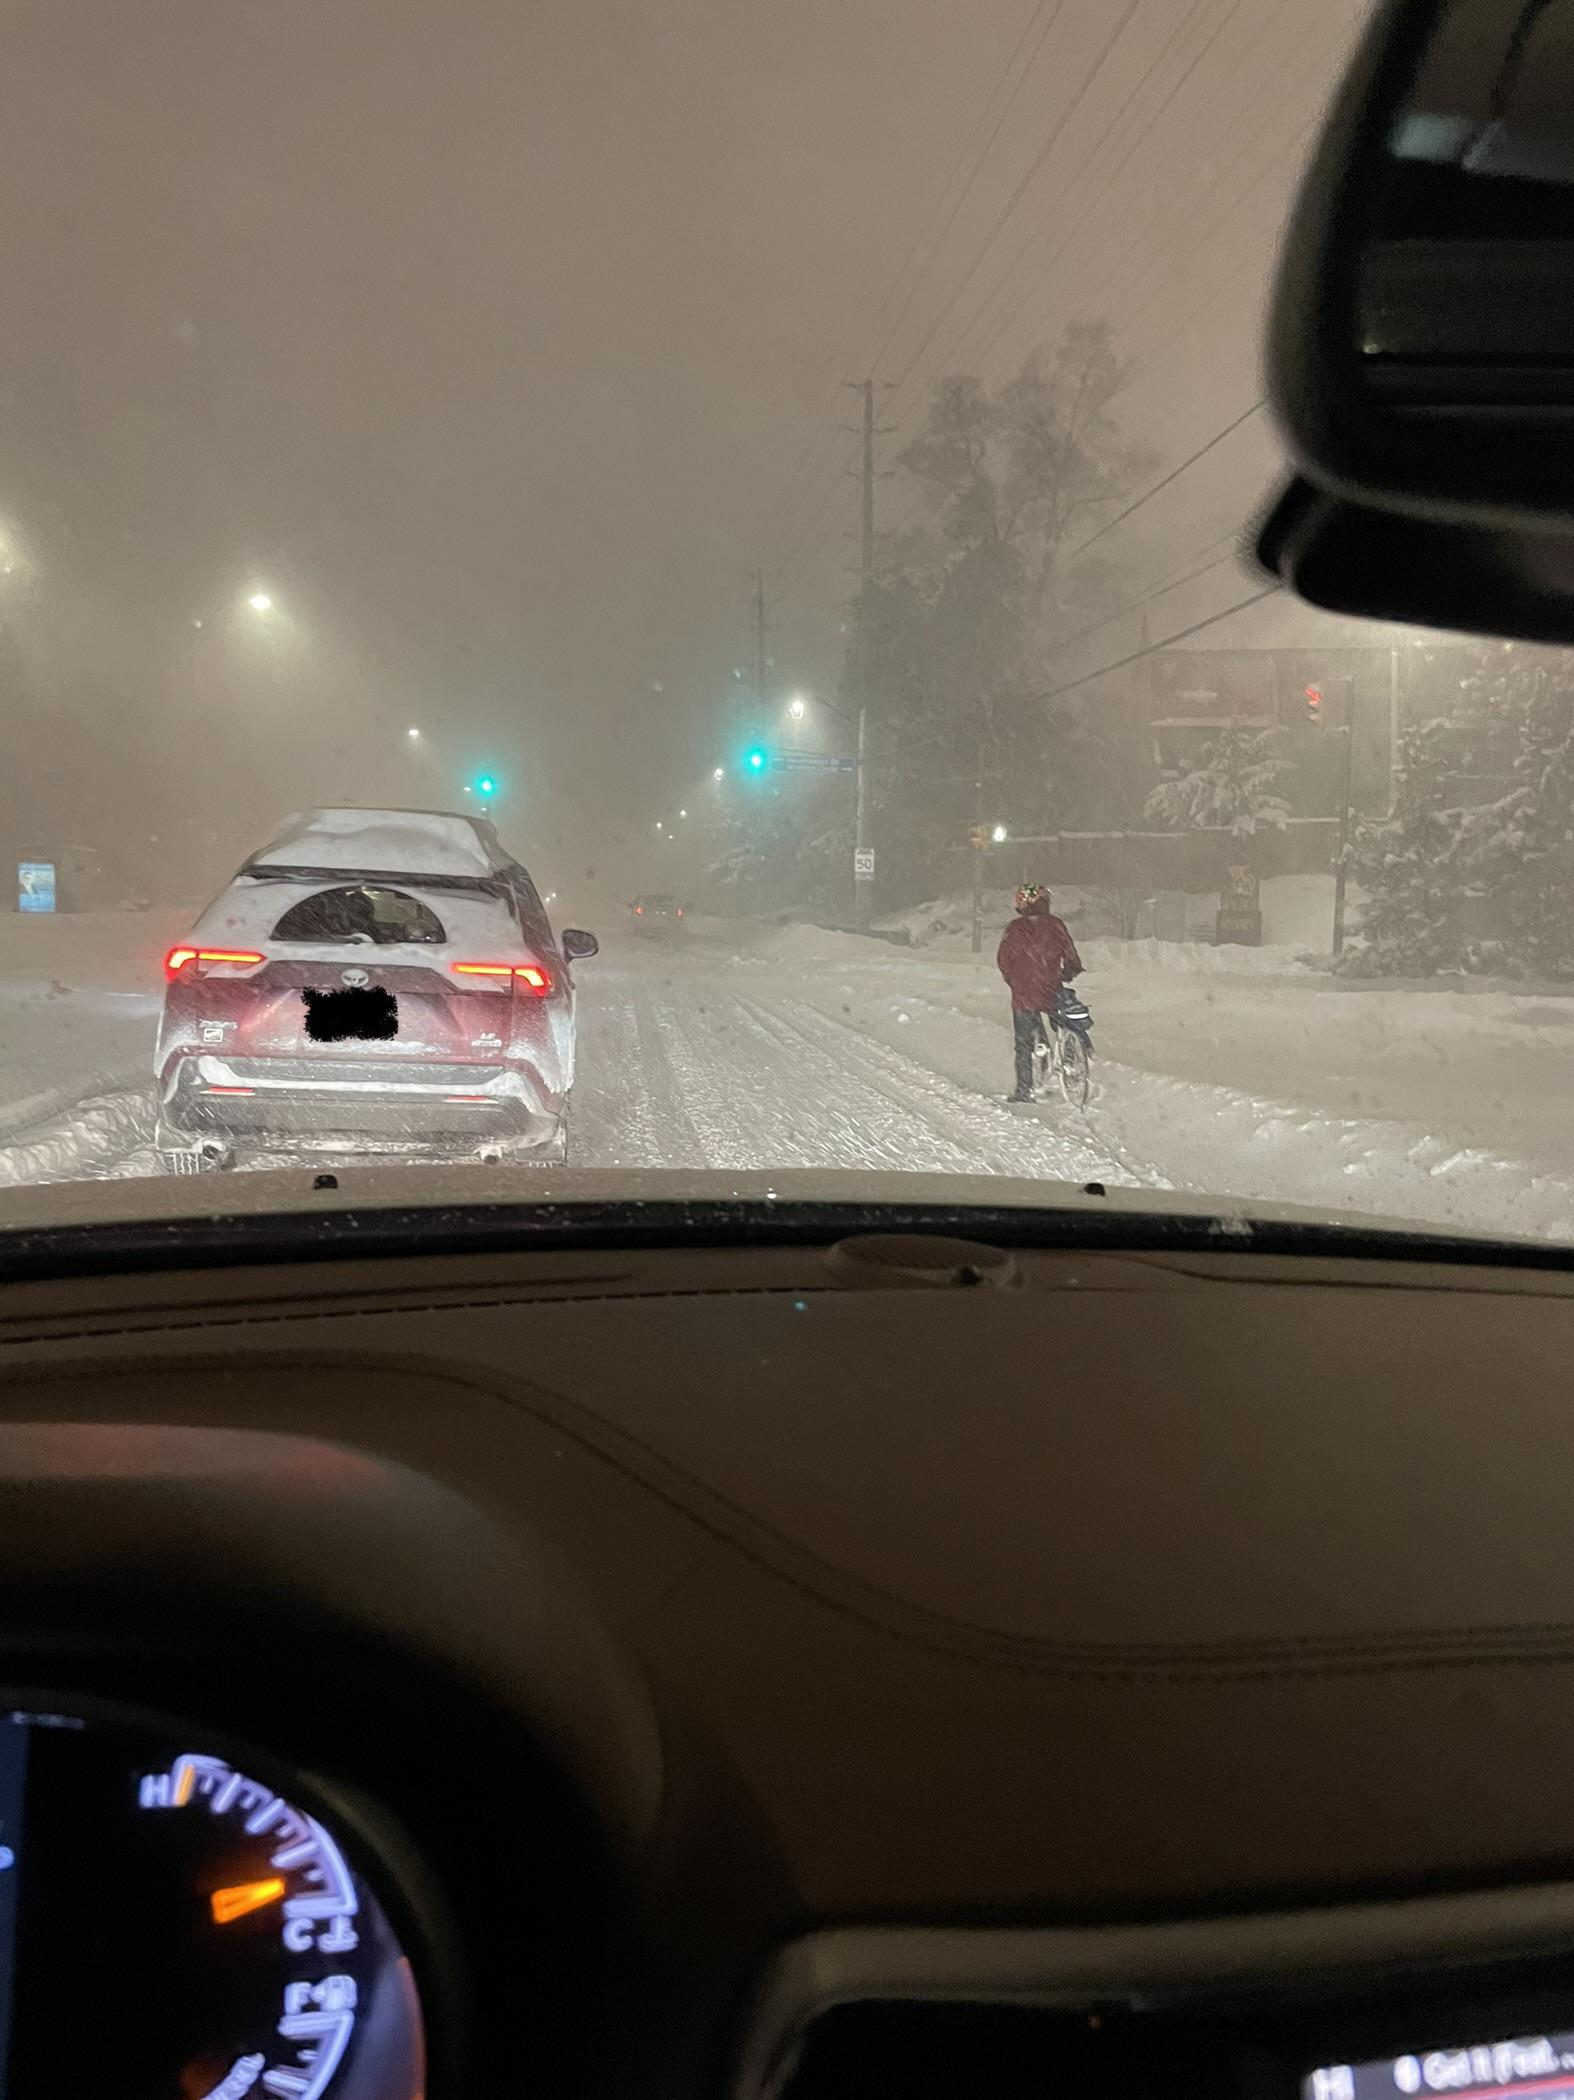
\includegraphics[width=0.8\linewidth]{images/bike_winter.jpg}
			\end{figure}
			
		\end{column}
		
		
		
	\end{columns}
\end{frame}




\begin{frame}
	
	\textbf{Active travel} - non-motorized mobility
	
	\vspace{2mm}
	
	e.g. walking and cycling, but also rollerblading, skateboarding, ice-skating, kick scooters, cross-country skiing, etc.
	
	\vspace{2mm}
	
	Can be for travelling to a specific location, or recreational travel not directed to a particular destination 

	\begin{figure}
		\centering
		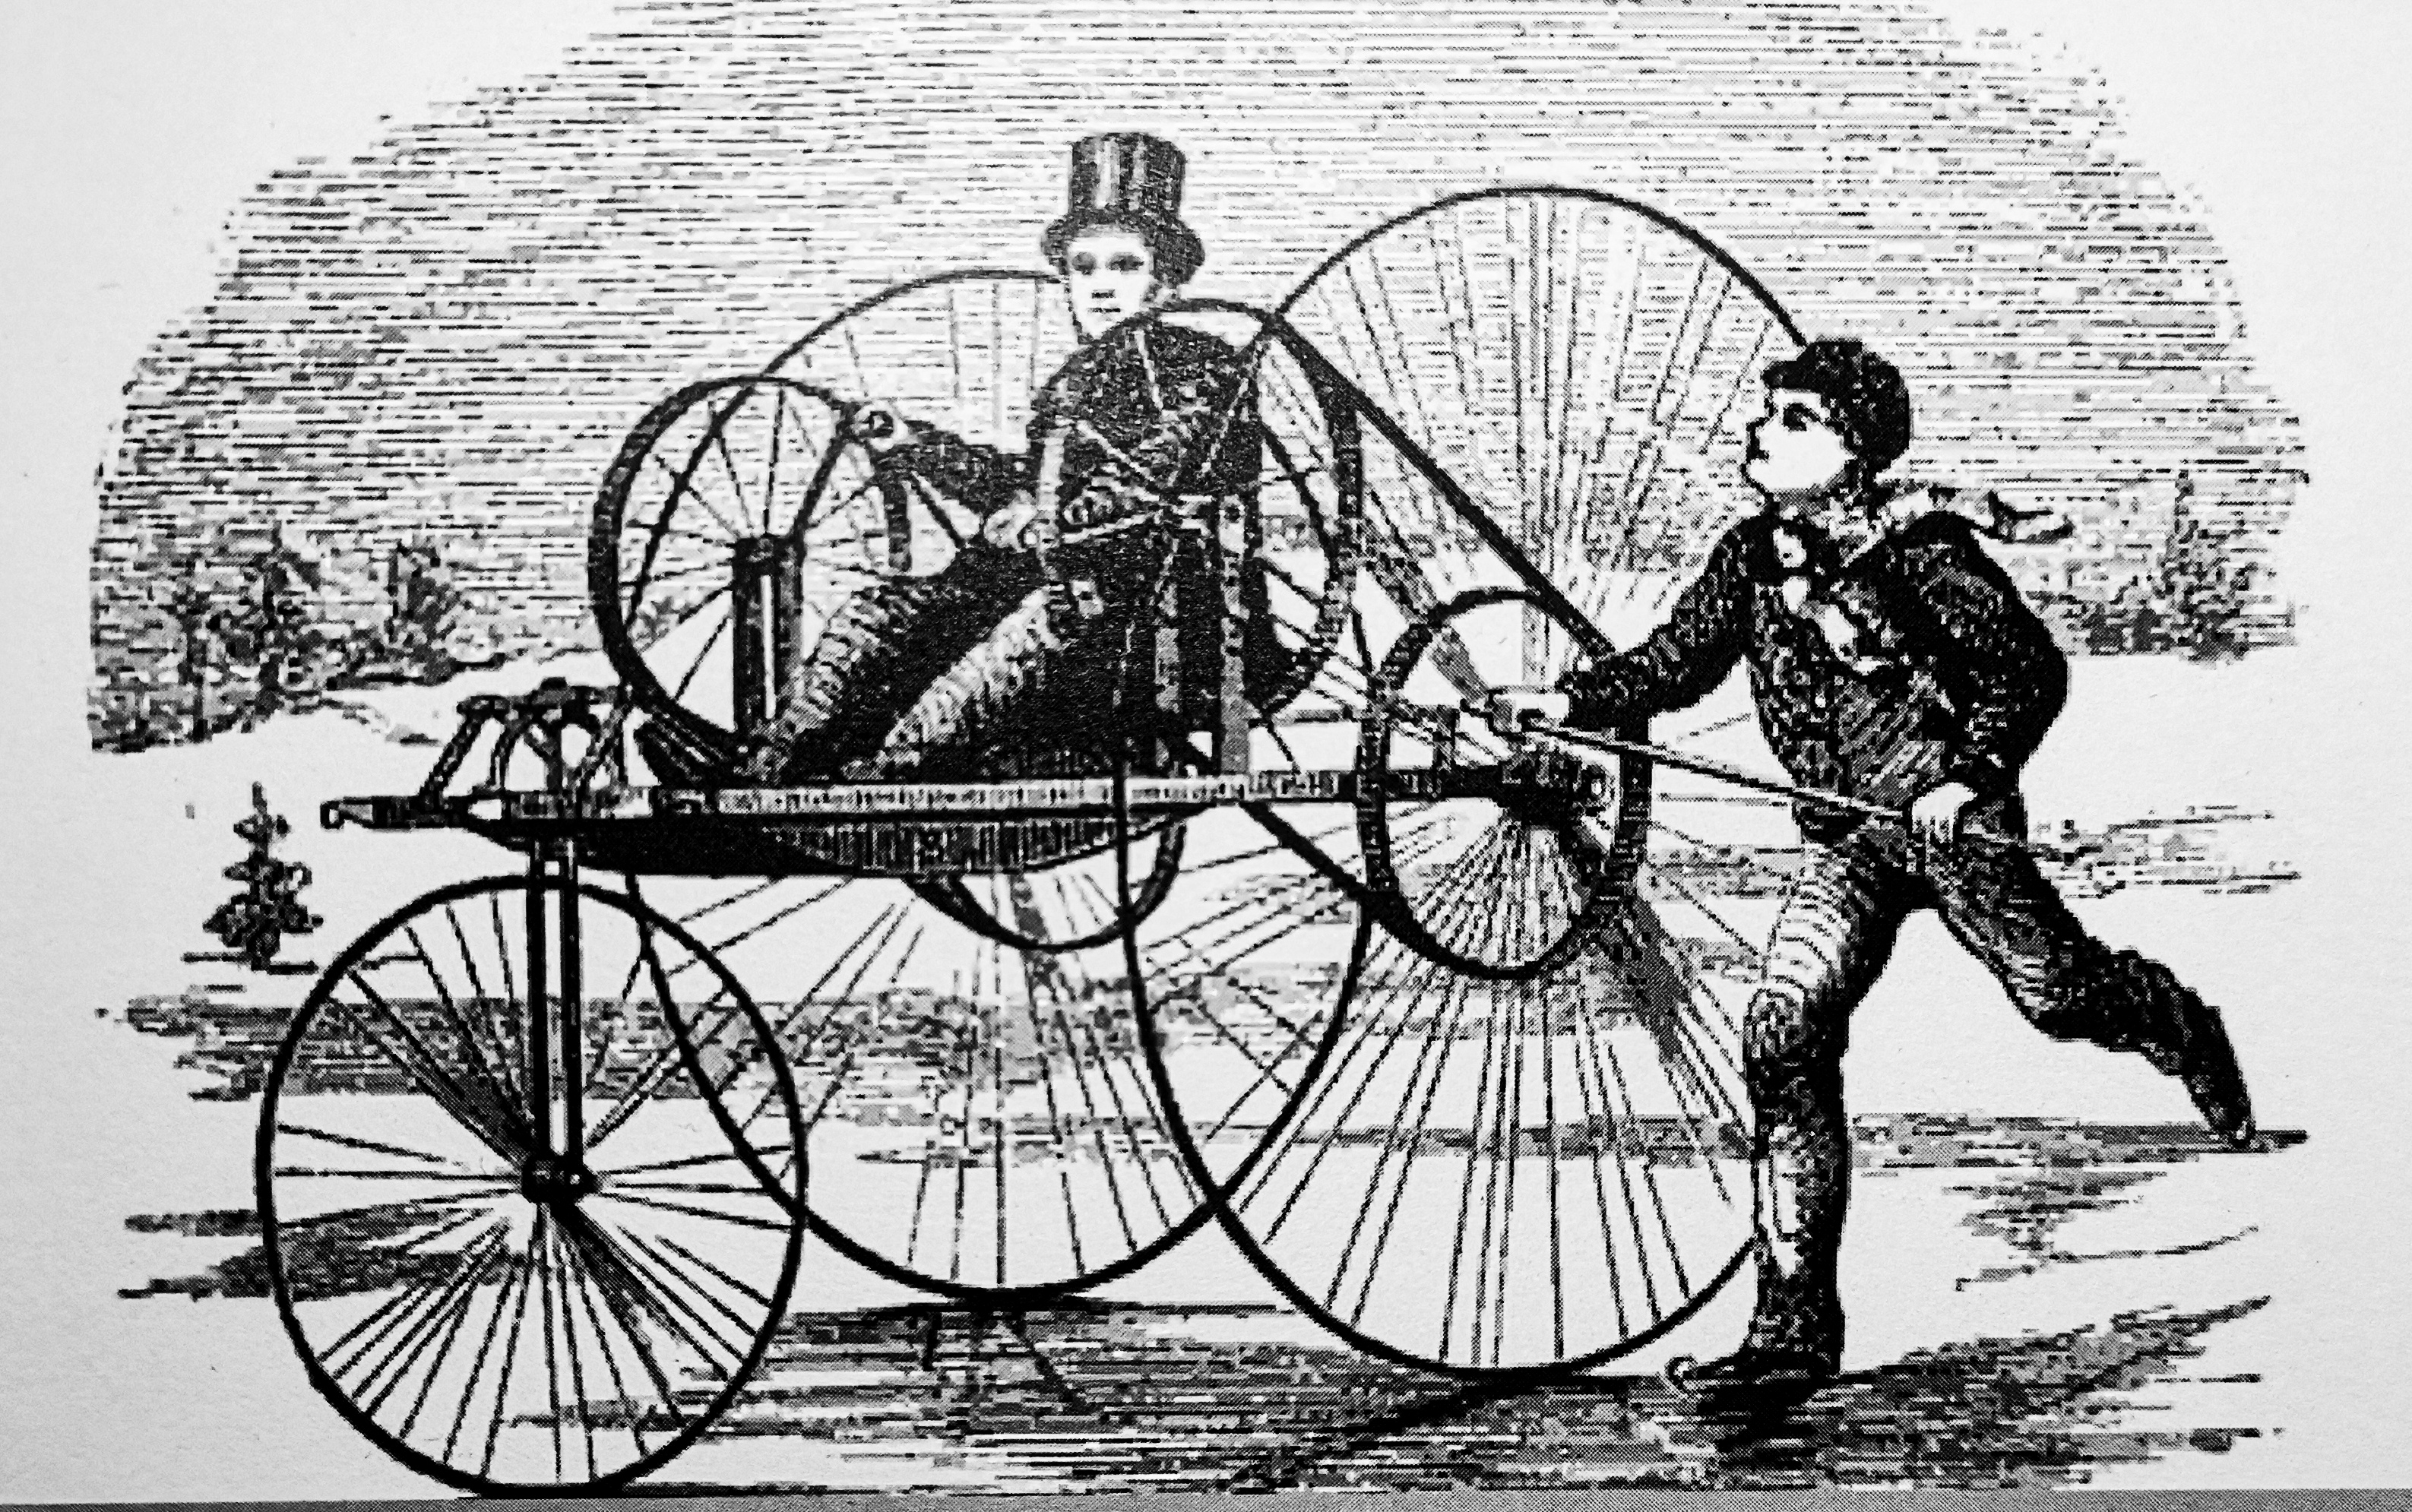
\includegraphics[width=0.55\linewidth]{images/velocipede.jpg}
	\end{figure}
		
\end{frame}




\begin{frame}
	
	\textbf{Benefits of Active Travel}
	
	\vspace{4mm}
	
	Can replace trips by other modes (driving, transit), meaning reduced congestion, pollution, GHG emissions, etc.
	
	\begin{figure}
		\centering
		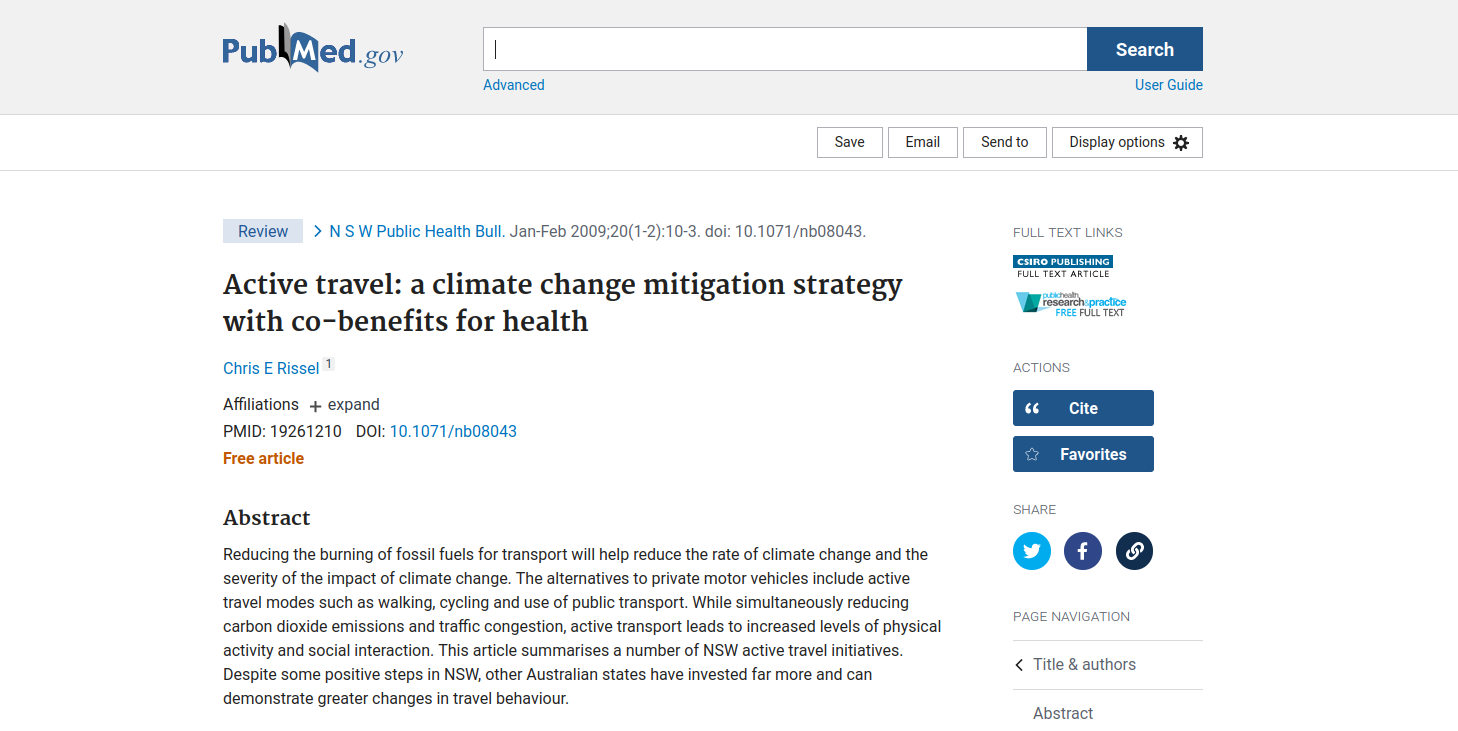
\includegraphics[width=0.7\linewidth]{images/active_travel_pollution.png}
	\end{figure}
	
	\tiny\url{https://pubmed.ncbi.nlm.nih.gov/19261210/}

\end{frame}



\begin{frame}
	
	\textbf{Benefits of Active Travel}
	
	\vspace{4mm}
	
	Plenty of research highlights health benefits of active travel, e.g. 
	
	\begin{figure}
		\centering
		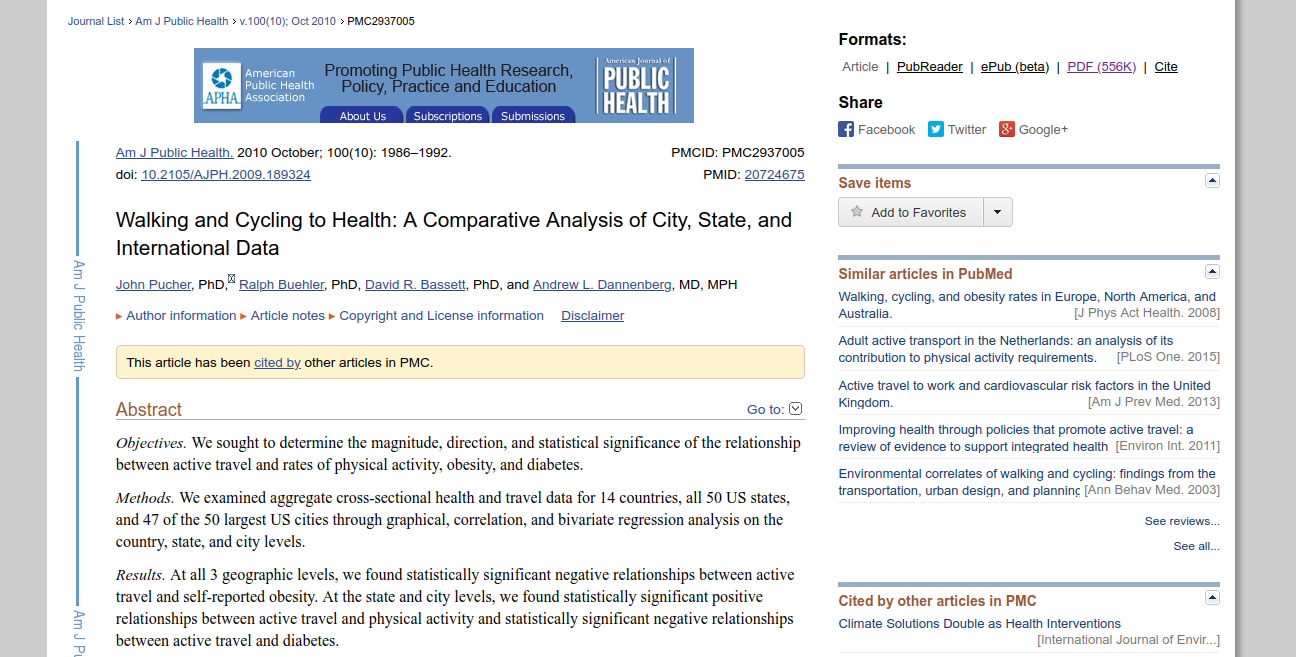
\includegraphics[width=1\linewidth]{images/health_ben_active_travel.png}
	\end{figure}
	
\end{frame}




\begin{frame}
	
	\textbf{Benefits of Active Travel}
	
	\vspace{4mm}
	
	Increased "enjoyment" or "satisfaction" of travel
	
	\begin{figure}
		\centering
		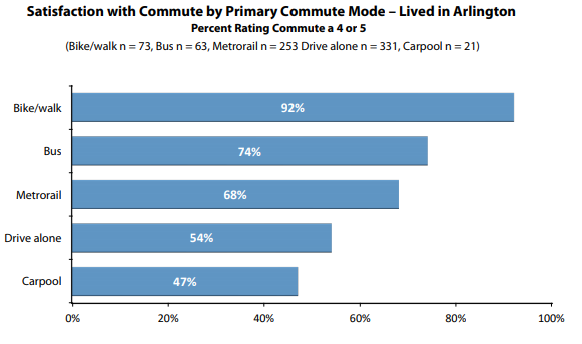
\includegraphics[width=0.7\linewidth]{images/mode_satisfaction.png}
	\end{figure}

	\tiny\url{https://mobilitylab.org/2020/09/29/the-pursuit-of-happiness-how-commute-mode-affects-commute-mood/}
	
\end{frame}



\begin{frame}
	
	\textbf{Benefits of Active Travel}
	
	\vspace{4mm}
	
	\small{"studies indicate that creating or improving active travel facilities generally has positive or non-significant economic impacts on retail"}
	
	\begin{figure}
		\centering
		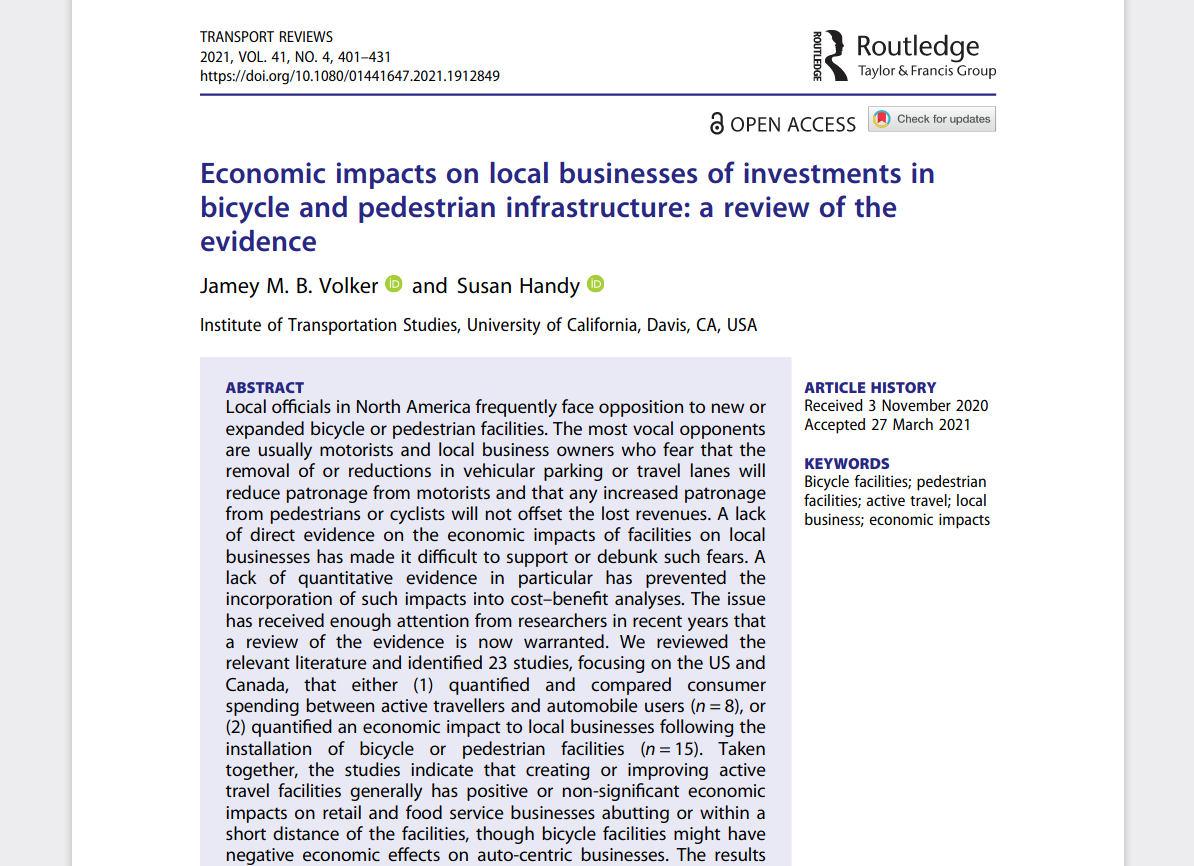
\includegraphics[width=0.6\linewidth]{images/economic_impacts_active_travel.png}
	\end{figure}
	
	\tiny\url{https://doi.org/10.1080/01441647.2021.1912849}
	
\end{frame}








\begin{frame}
	\begin{columns}
		\begin{column}{0.5\textwidth}
			
			\textbf{What deters active travel?}
			
			\vspace{8mm}
			
			\tiny{Image by Karl Jilg, commissioned by the Swedish Road Administration in 2014}
				
			\tiny\url{https://archive.attn.com/stories/17066/illustration-nails-pedestrian-problem-cities}
			
		\end{column}
		
		\begin{column}{0.5\textwidth}
			\begin{figure}
				\centering
				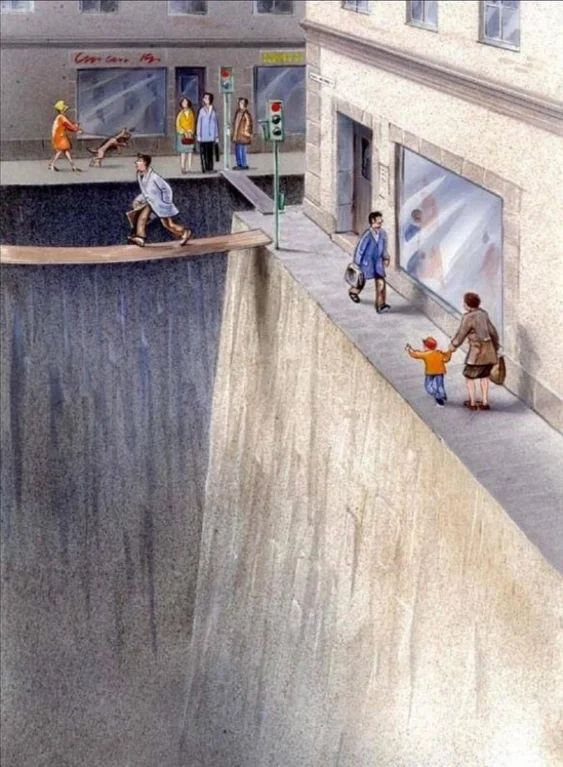
\includegraphics[width=0.9\linewidth]{images/deter_active_travel.jpg}
			\end{figure}
			
		\end{column}
		
		
		
	\end{columns}
\end{frame}








%
%
%
%\begin{frame}
%	
%	Avenues vs Arterials:
%	
%	
%\end{frame}
%



\begin{frame}
	
	\textbf{Vision Zero}
	
	\vspace{2mm}
	
	\begin{itemize}
		\item Road safety strategies aimed reducing road fatalities to zero
		\item Started in Sweden in 1997 and has since been implimented in hundreds of cities
		\item Focus on design of infrastructure, and responsibility of road/street engineers and designers
		\item Accepting inevitability of human error - making accidents less severe
	\end{itemize}

	\begin{figure}
		\centering
		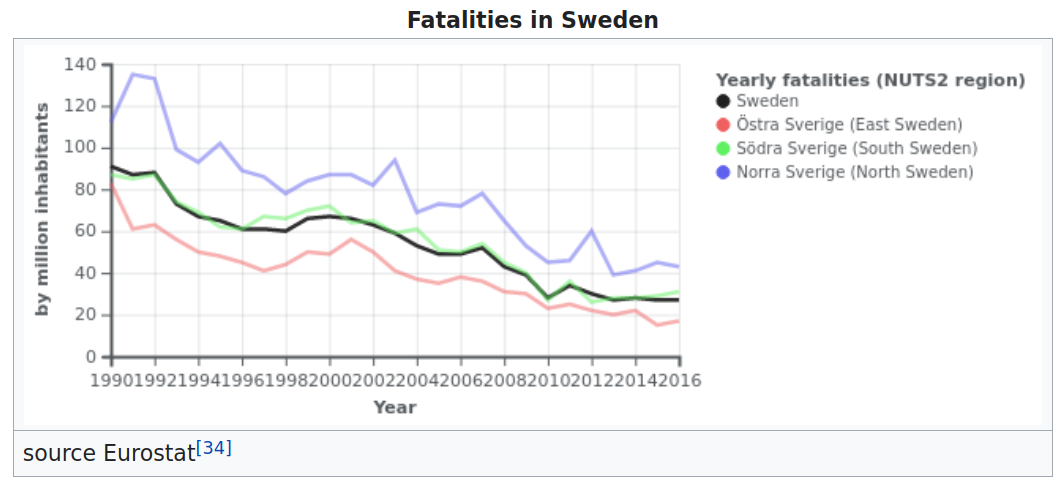
\includegraphics[width=0.75\linewidth]{images/sweden_road_fatalities.png}
		
	\end{figure}
	\tiny{\url{https://en.wikipedia.org/wiki/Vision_Zero}}


	
\end{frame}




\begin{frame}
	
	Vision Zero initiatives in Toronto formally began in 2016
		
	\begin{figure}
		\centering
		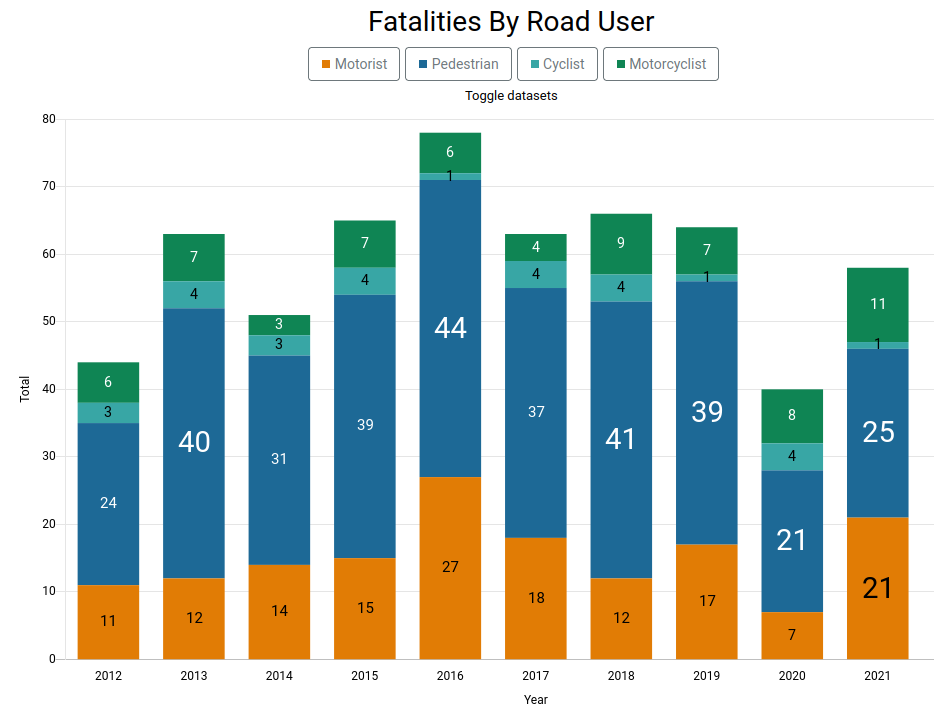
\includegraphics[width=0.55\linewidth]{images/vision_zero_deaths.png}
		
	\end{figure}

	\small
	\begin{itemize}
		\item "83\% of KSI (Killed or Seriously Injured) collisions happen on arterial roadways"
		\item "Vulnerable road users have a 95\% likelihood of death
		in a collision at 60 km/hr, while at 40 km/hr the likelihood of death is reduced to 30\%"
	\end{itemize}

	\tiny{\url{https://www.toronto.ca/legdocs/mmis/2019/ie/bgrd/backgroundfile-134964.pdf}}
	
\end{frame}



\begin{frame}
	
	Many (arterial) roads are predominately designed for cars:
	
	\begin{figure}
		\centering
		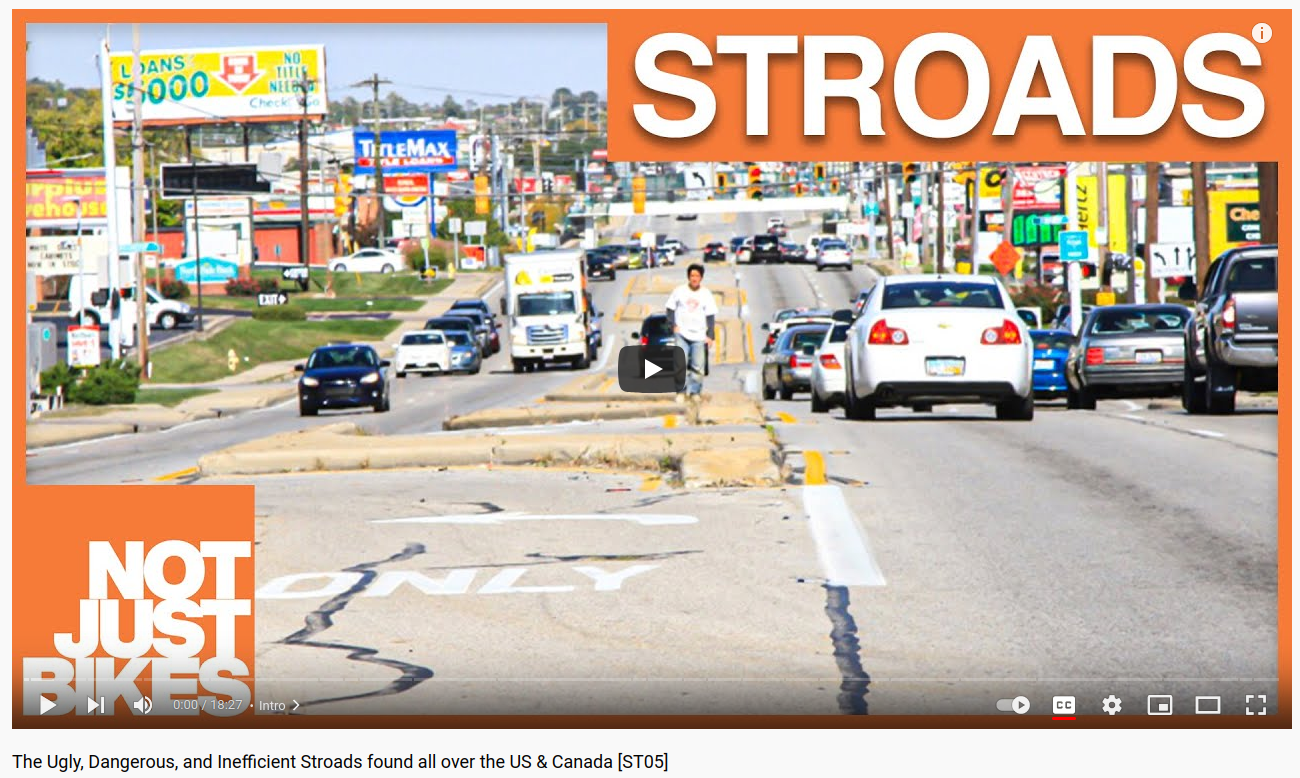
\includegraphics[width=0.85\linewidth]{images/stroads.png}
		
	\end{figure}
	\tiny{\url{https://www.youtube.com/watch?v=ORzNZUeUHAM}}
	
\end{frame}



\begin{frame}
	
	Toronto's Road Classification System:
	
	\begin{figure}
		\centering
		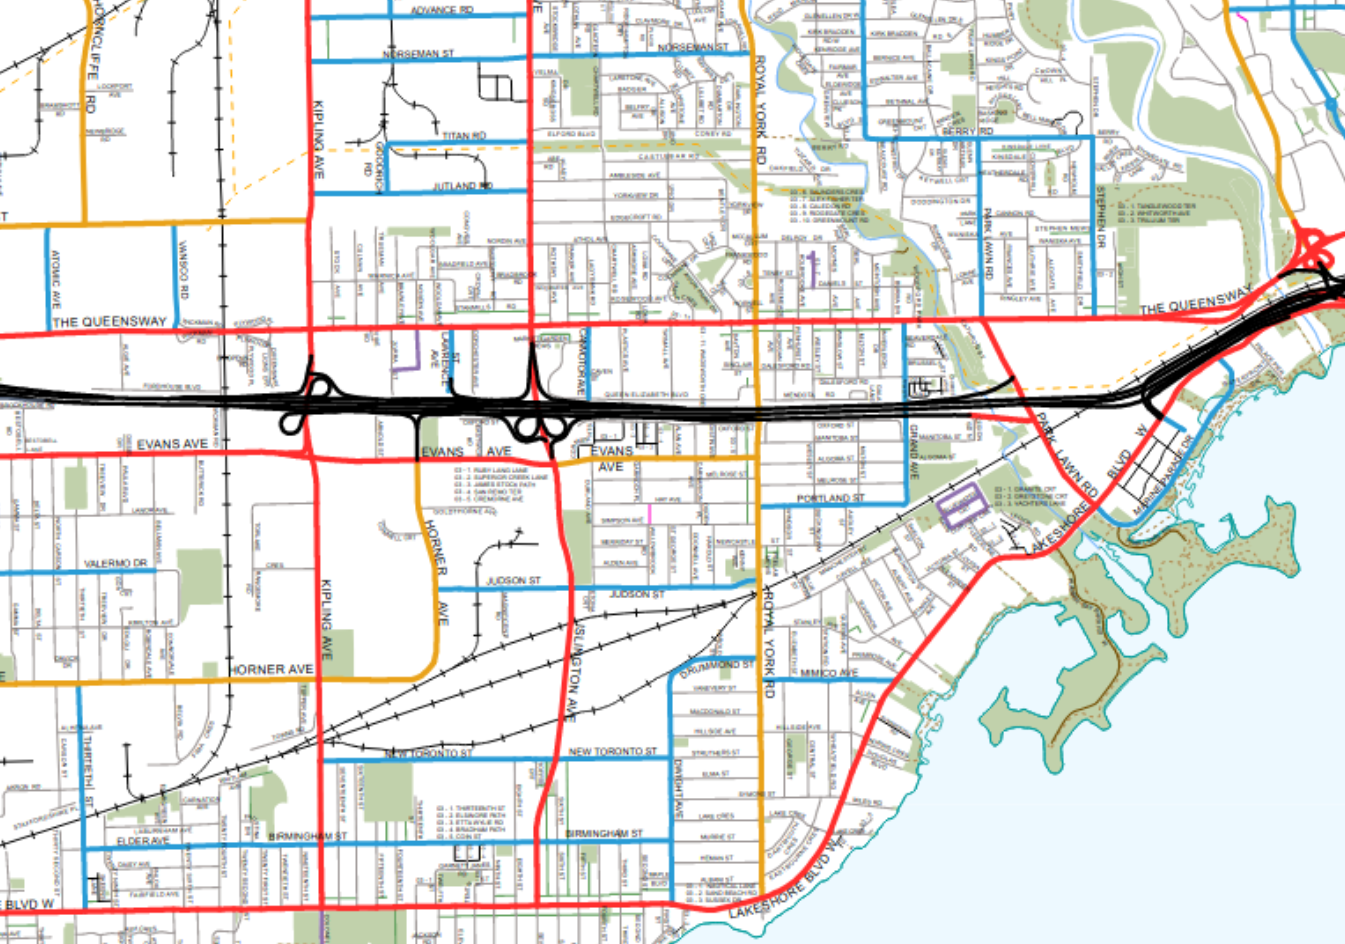
\includegraphics[width=0.75\linewidth]{images/tor_road_heir.png}
		
	\end{figure}
	\tiny{\url{https://www.toronto.ca/services-payments/streets-parking-transportation/traffic-management/road-classification-system/}}
	
\end{frame}



\begin{frame}
	
	Toronto's Road Classification System:
	
	\begin{figure}
		\centering
		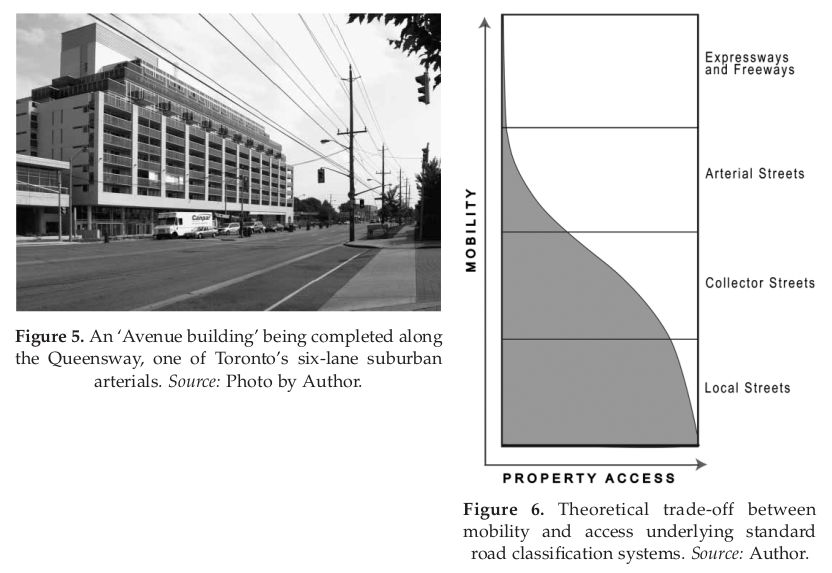
\includegraphics[width=0.75\linewidth]{images/road_heir_hes.png}
		
	\end{figure}
	\tiny Image from Hess (2009)
	
	
	
\end{frame}



\begin{frame}
	
	\textbf{Safer streets:} Lower speed limits
	
	\begin{figure}
		\centering
		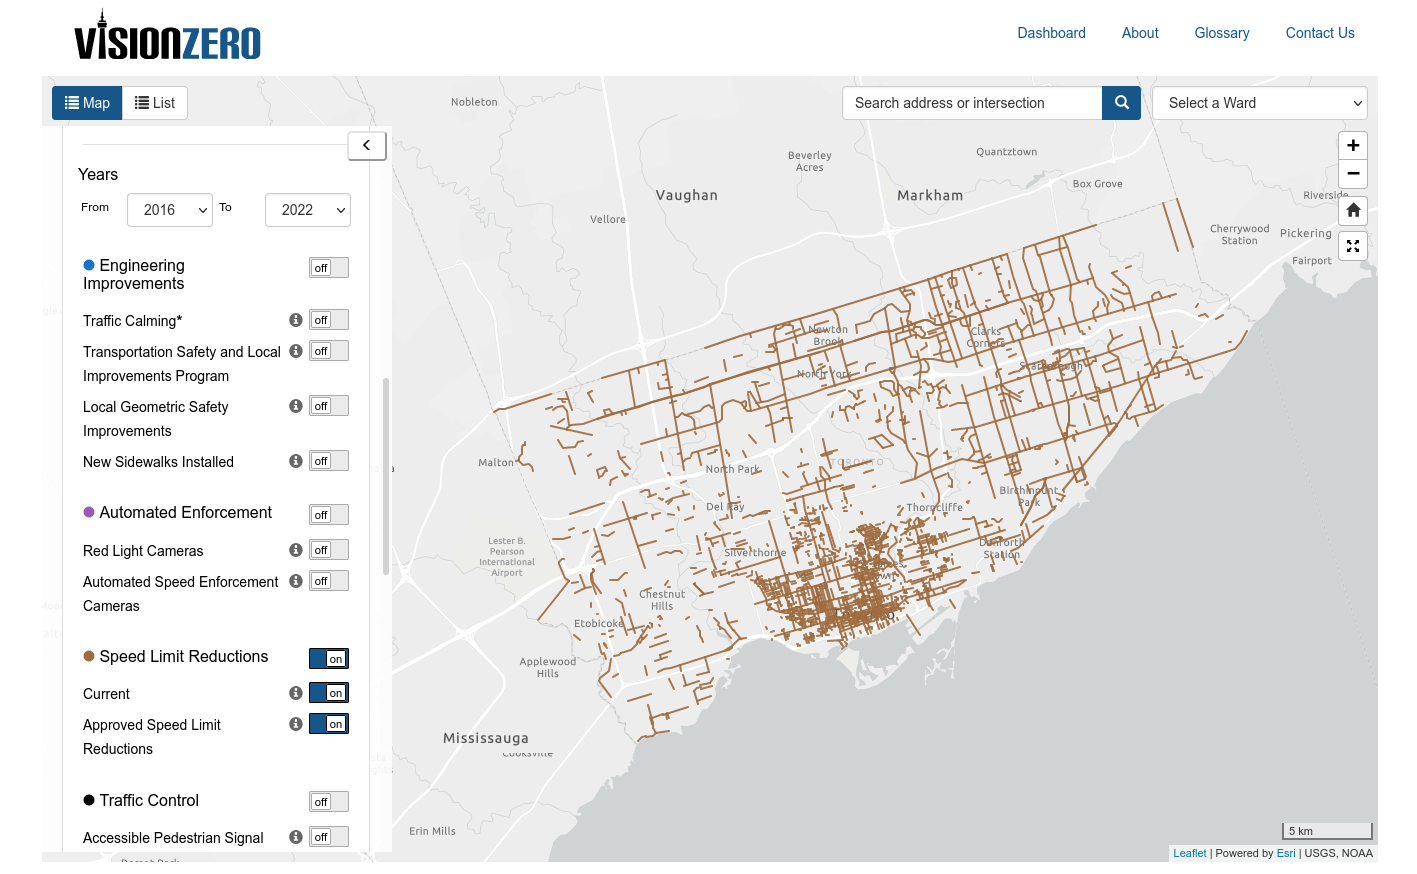
\includegraphics[width=0.75\linewidth]{images/speed_limit_reduction.png}
	\end{figure}

	\tiny\url{https://www.toronto.ca/services-payments/streets-parking-transportation/road-safety/vision-zero/safety-measures-and-mapping/}
	
\end{frame}




\begin{frame}
	
	\textbf{Safer streets:} Automated enforcement
	
	\begin{figure}
		\centering
		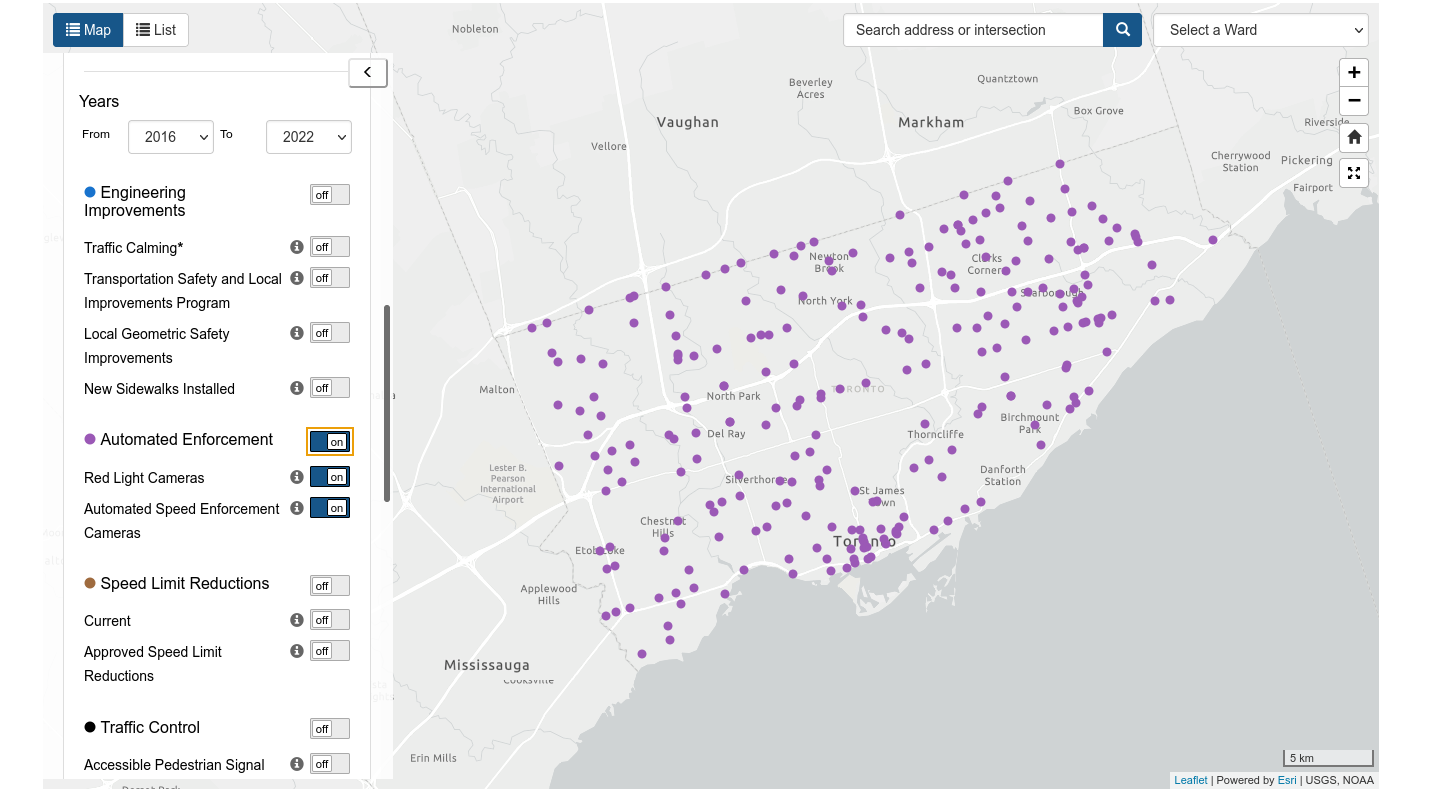
\includegraphics[width=0.75\linewidth]{images/automated_enforcement.png}
	\end{figure}
	
	\tiny\url{https://www.toronto.ca/services-payments/streets-parking-transportation/road-safety/vision-zero/safety-measures-and-mapping/}
	
\end{frame}




% traffic signals and pedestrian crossings


\begin{frame}
	
	\textbf{Safer streets:} Pedestrian Crossovers
	
	\begin{figure}
		\centering
		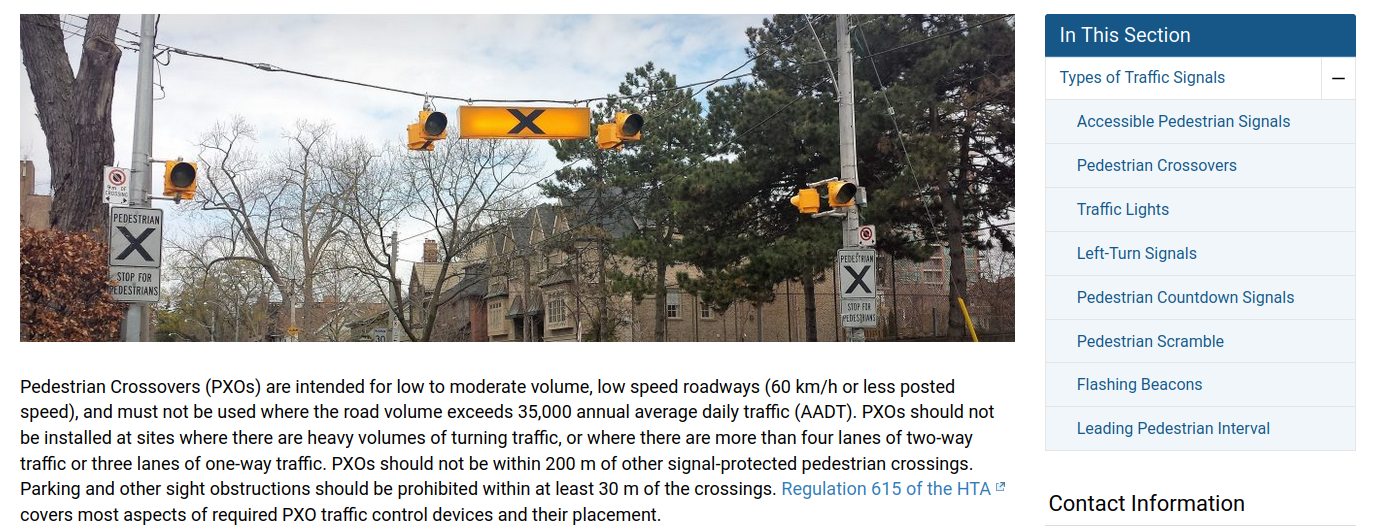
\includegraphics[width=1\linewidth]{images/pedestrian_pxo.png}
	\end{figure}
	
	\tiny\url{https://www.toronto.ca/services-payments/streets-parking-transportation/traffic-management/traffic-signals-street-signs/types-of-traffic-signals/pedestrian-crossovers/}
	
	
\end{frame}



\begin{frame}
	
	\textbf{Safer streets:} Raised Pedestrian Crossings
	
	\begin{figure}
		\centering
		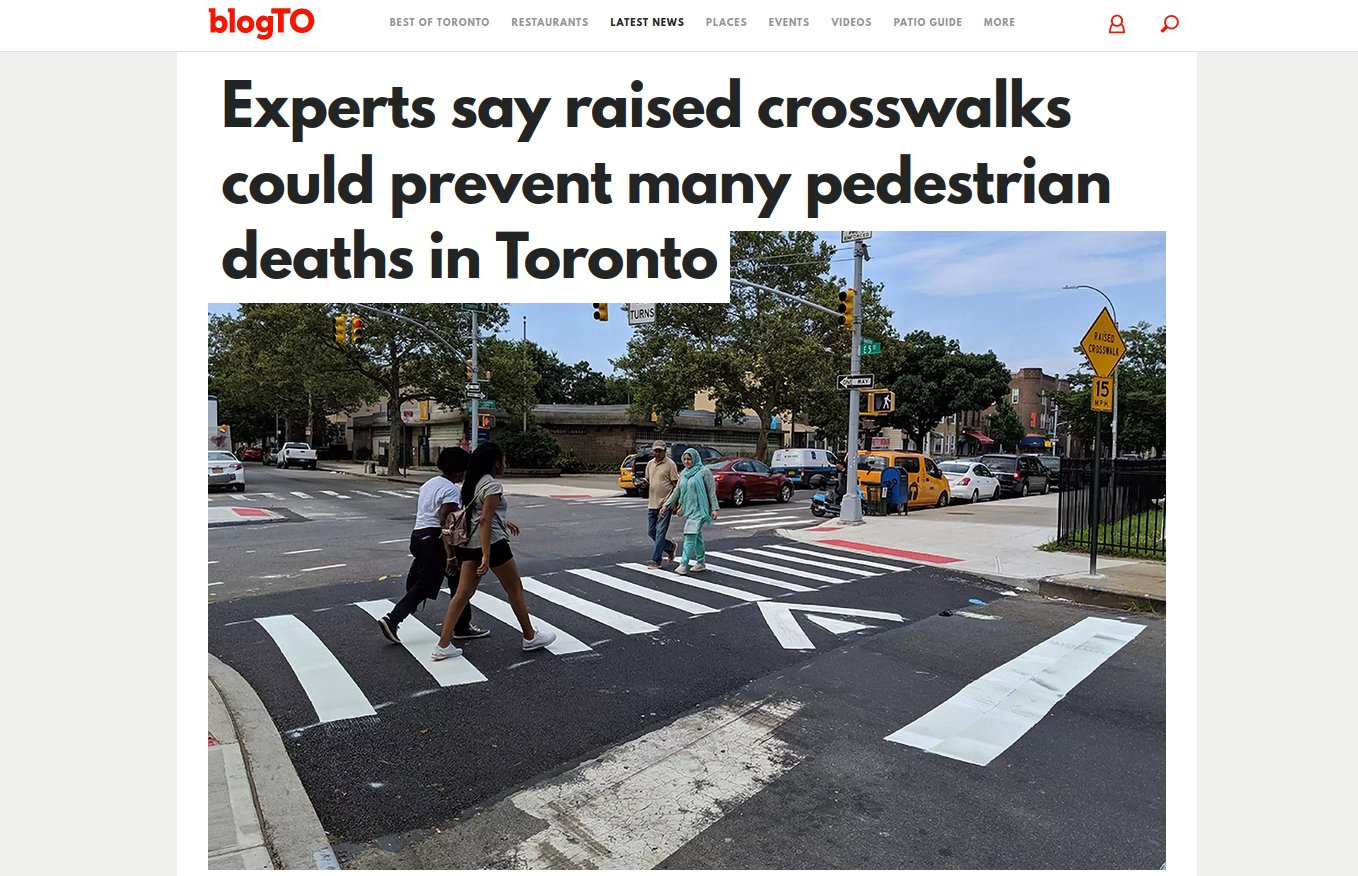
\includegraphics[width=0.8\linewidth]{images/raised_crossings.png}
	\end{figure}
	
	\tiny\url{https://www.blogto.com/city/2022/01/experts-say-raised-crosswalks-could-prevent-many-pedestrian-deaths-toronto/}
	
	
\end{frame}




\begin{frame}
	
	\textbf{Safer streets:} Leading Pedestrian Interval (i.e. Pedestrian Head Start Signal)
	
	\begin{figure}
		\centering
		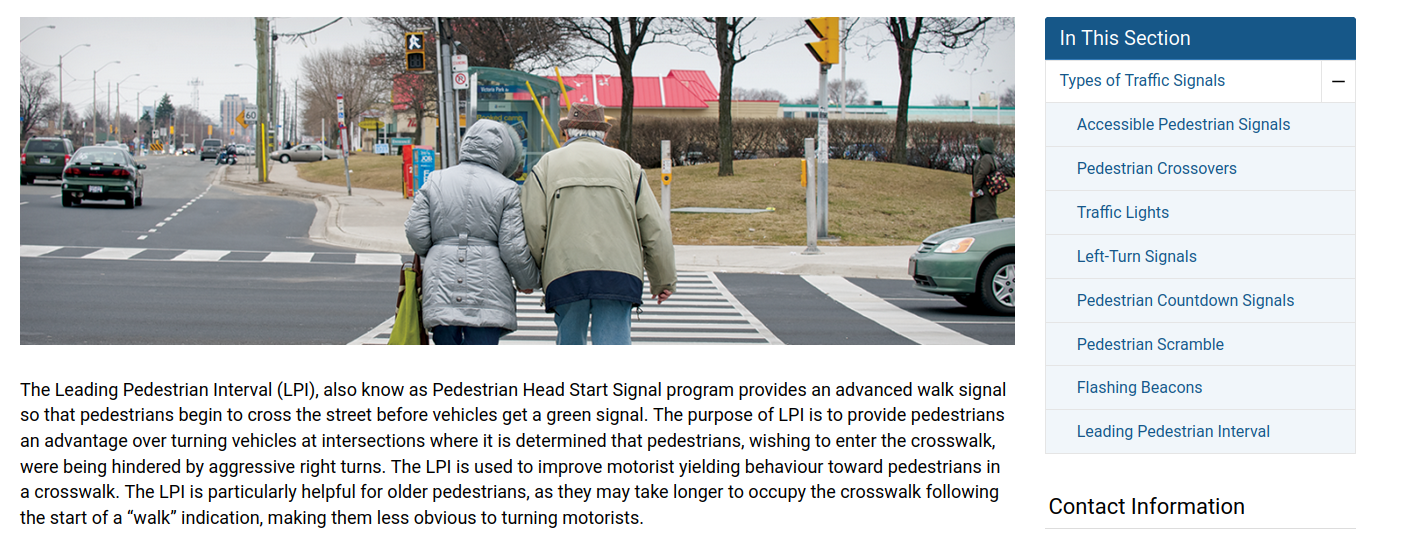
\includegraphics[width=1\linewidth]{images/pedestrian_leading.png}
	\end{figure}
	
	\tiny\url{https://www.toronto.ca/services-payments/streets-parking-transportation/traffic-management/traffic-signals-street-signs/types-of-traffic-signals/leading-pedestrian-interval-phase/}
	
\end{frame}



\begin{frame}
	
	\textbf{Safer streets:} Traffic calming infrastructure / engineering improvements
	
	\begin{figure}
		\centering
		\includegraphics[width=0.665\linewidth]{images/wellington.jpg}
	\end{figure}

	\tiny\url{https://www.toronto.ca/services-payments/streets-parking-transportation/road-safety/vision-zero/safety-initiatives/reduced-crossing-distances/}
	
	\tiny\url{https://www.tcat.ca/project/saferstreetsnearschools-getting-started/traditional-traffic-calming-measures/}
	
\end{frame}








\begin{frame}
	
	\textbf{Safer streets:} Traffic calming infrastructure / engineering improvements
	
	\vspace{2mm}
	
	e.g. Glen Road in Rosedale
	
		\begin{columns}
		\begin{column}{0.5\textwidth}
			\begin{figure}
				\centering
				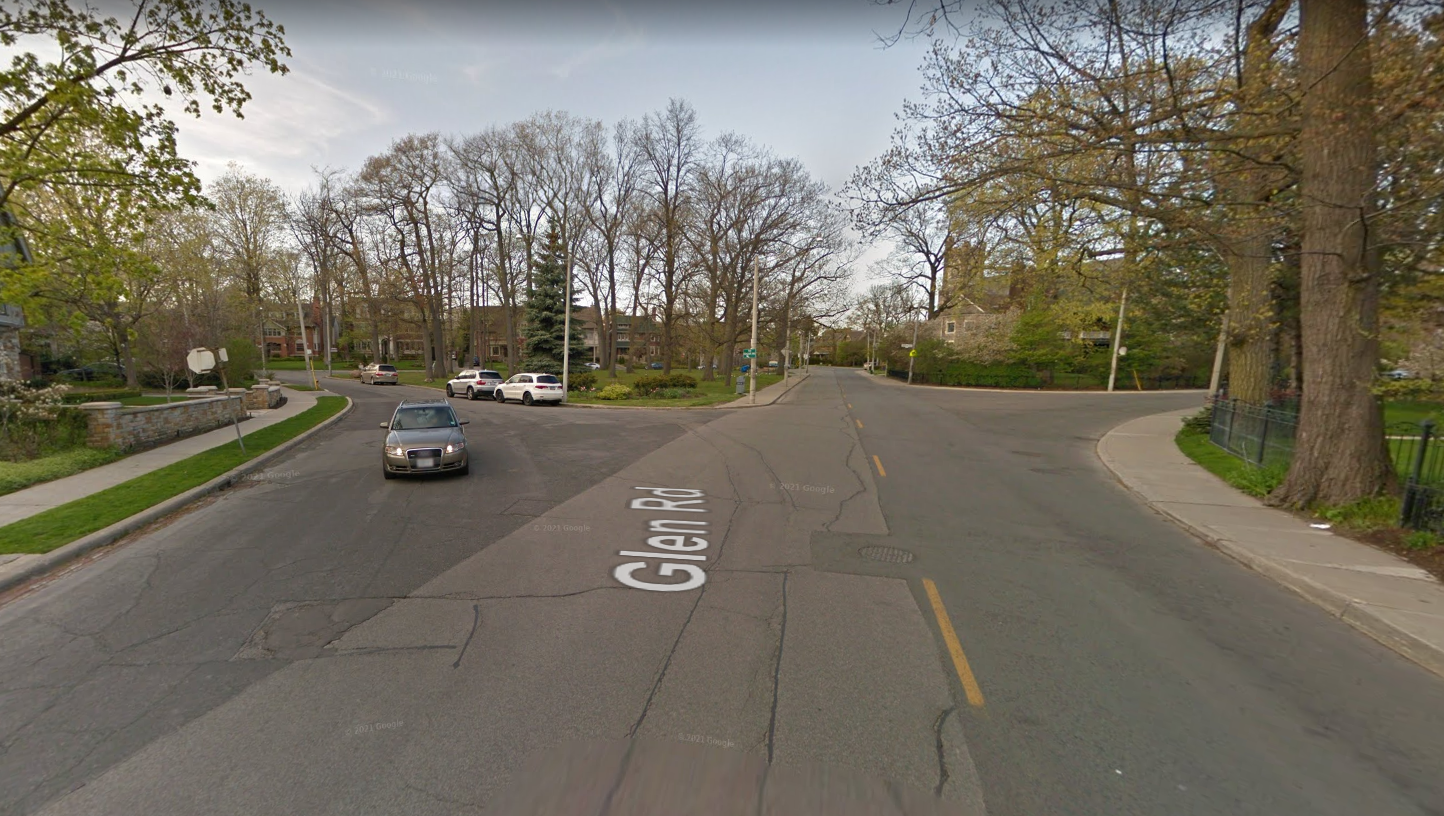
\includegraphics[width=1.1\linewidth]{images/glen_2016.png}
			\end{figure}
			
			
		\end{column}
		
		\begin{column}{0.5\textwidth}
			\begin{figure}
				\centering
				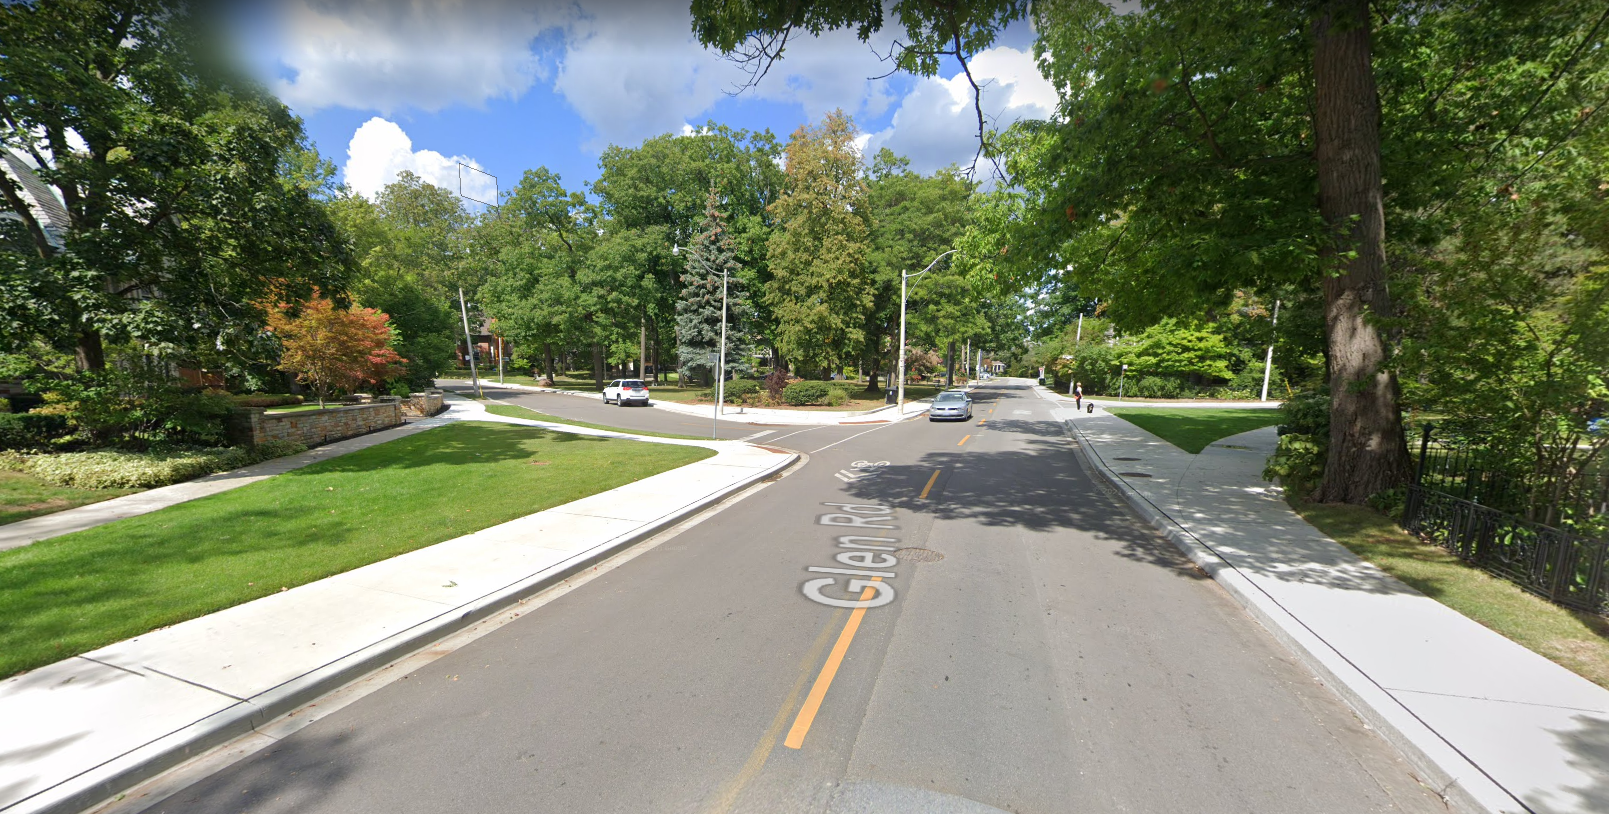
\includegraphics[width=1.2\linewidth]{images/glen_2021.png}
			\end{figure}
			
		\end{column}
		
		
		
	\end{columns}

	\tiny{Images: Google Maps}
	
	\vspace{2mm}
	
	\tiny\url{https://www.toronto.ca/services-payments/streets-parking-transportation/road-safety/vision-zero/safety-initiatives/reduced-crossing-distances/}
	
	\tiny\url{https://www.tcat.ca/project/saferstreetsnearschools-getting-started/traditional-traffic-calming-measures/}
	
	
	
\end{frame}





% raised ped crossing

% narrower car lanes - snow example

% chicanes, curb extensions, crossing islands

% city example - e.g. site intersection "diet"

% pavement vs asphalt

% woonerf








\begin{frame}
	
	\textbf{Reducing barriers to cycling:} Building safe and comfortable infrastructure 
	
	\begin{figure}
		\centering
		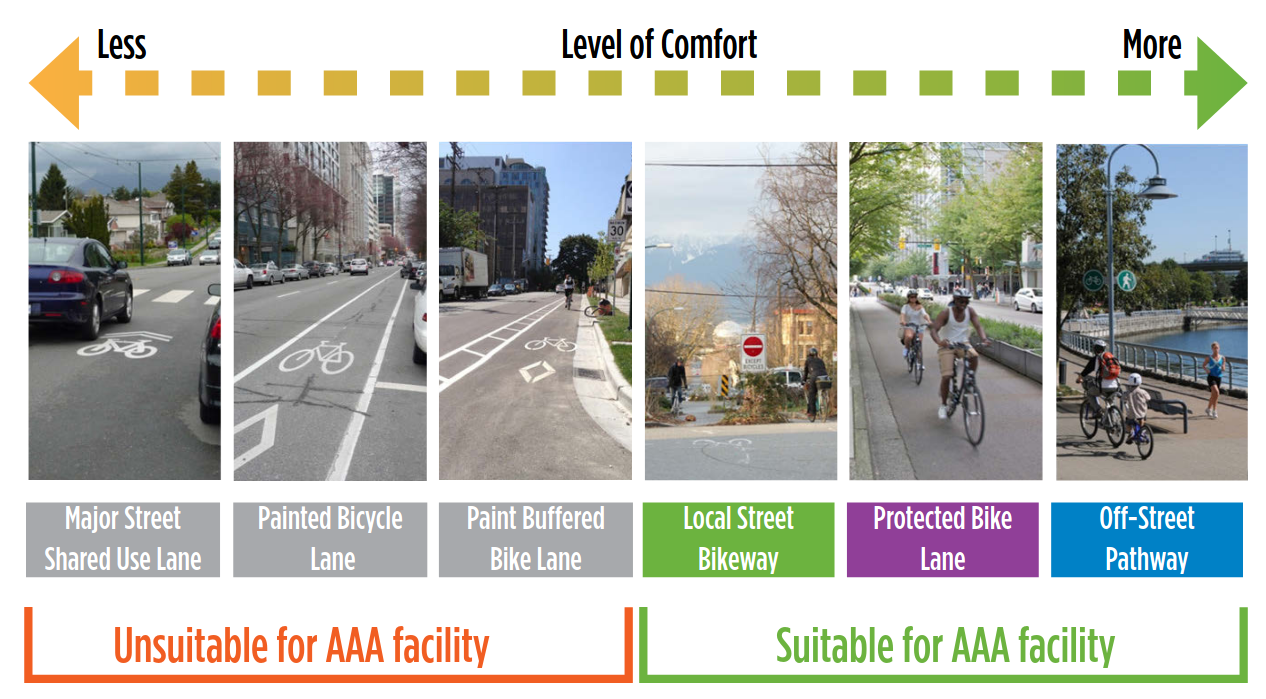
\includegraphics[width=0.85\linewidth]{images/bike_inf_comfort.png}
	\end{figure}

	\small{"The City of Vancouver has a vision to make cycling safe,
		convenient, comfortable and fun for all ages and abilities
		(AAA)"}
	\vspace{2mm}
	
	\tiny\url{https://vancouver.ca/files/cov/design-guidelines-for-all-ages-and-abilities-cycling-routes.pdf}
	
\end{frame}





\begin{frame}
	
	\textbf{Induced demand, not just for cars!}
	
	\begin{figure}
		\centering
		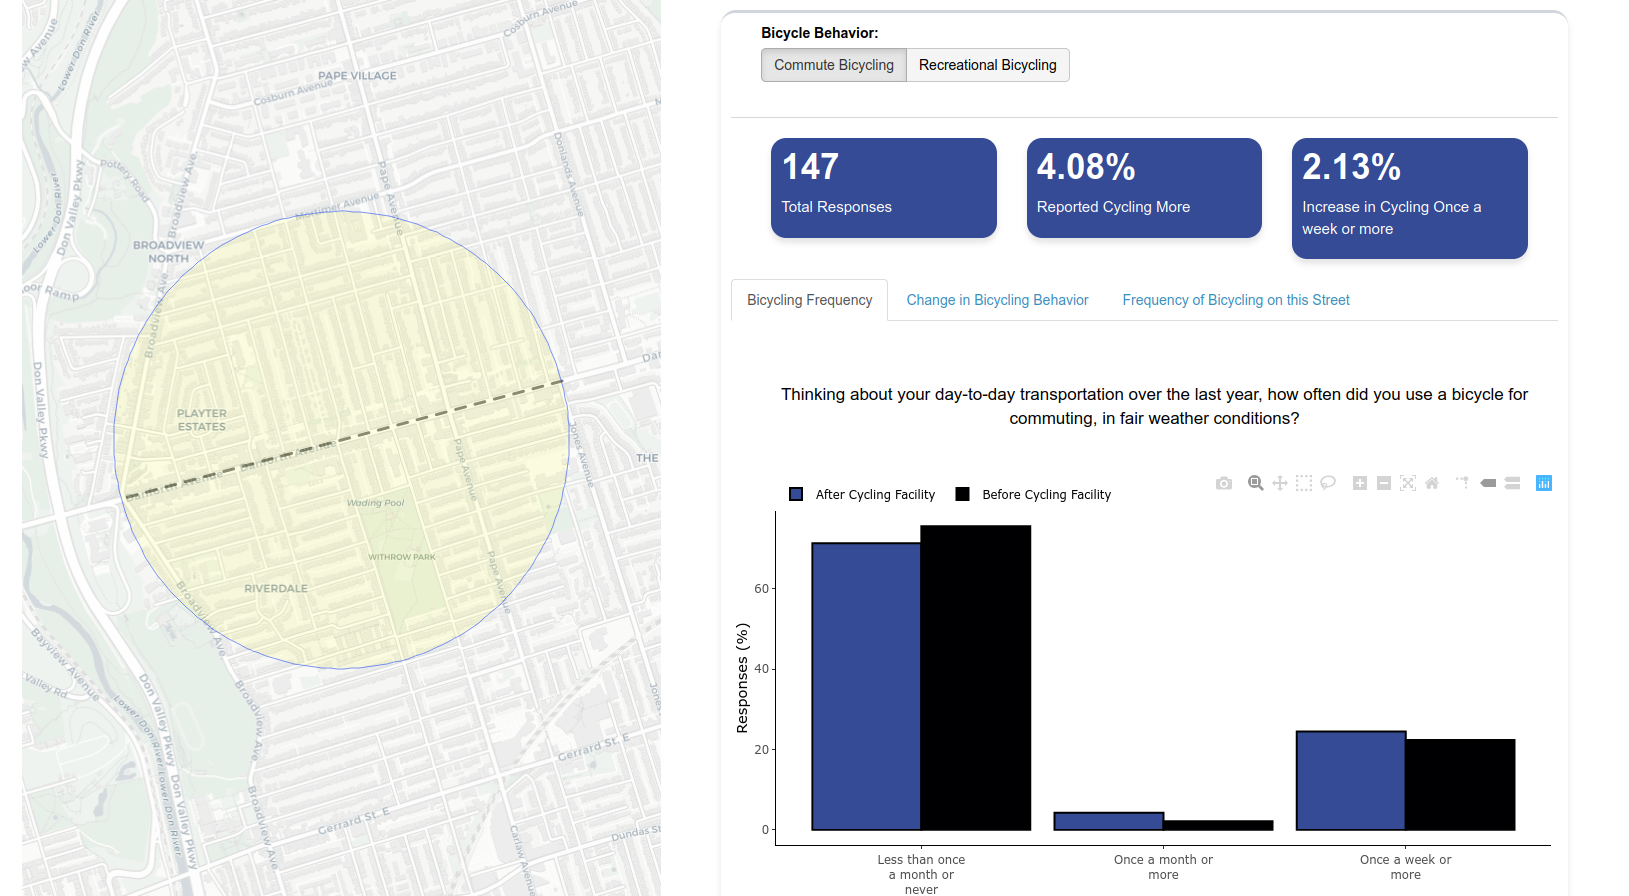
\includegraphics[width=0.95\linewidth]{images/ryerson_cycle_danforth.png}
	\end{figure}
	
	\tiny\url{https://transformlab.shinyapps.io/CyclingInGTHA/}
	
\end{frame}





\begin{frame}
	
	\textbf{Reducing barriers to cycling:} Available and safe bicycle parkring
	
	\begin{figure}
		\centering
		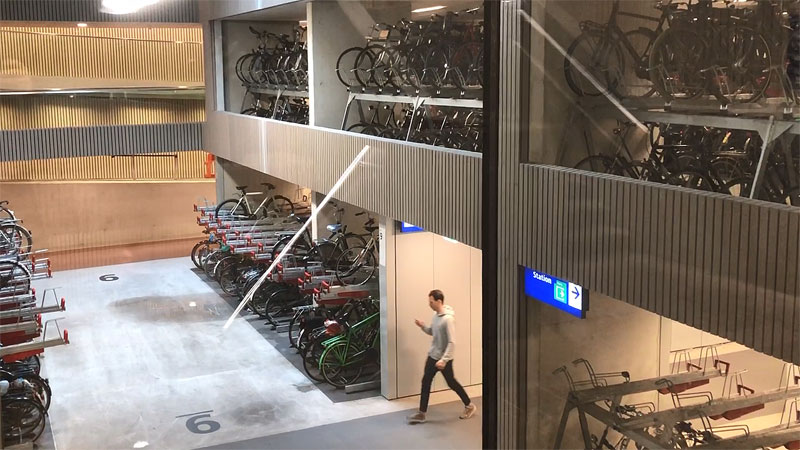
\includegraphics[width=0.85\linewidth]{images/bike_parking_neth.jpg}
	\end{figure}
	
	\tiny\url{https://bicycledutch.wordpress.com/2019/08/20/finally-fully-open-utrechts-huge-bicycle-parking-garage/}
	
\end{frame}



\begin{frame}
	
	\textbf{Reducing barriers to cycling:} Bike escalators in Norway
	
	\begin{figure}
		\centering
		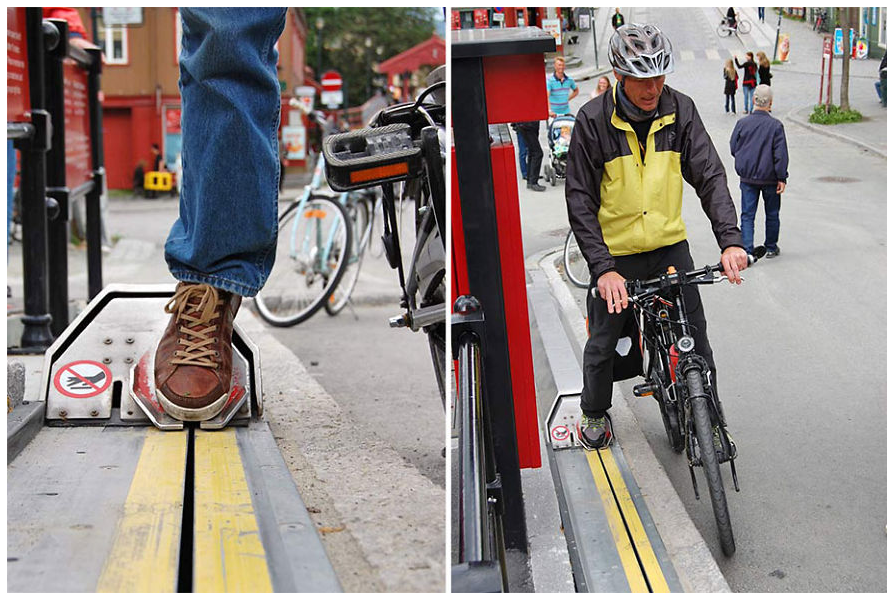
\includegraphics[width=0.85\linewidth]{images/norway_bike_escalator.png}
	\end{figure}
	
	\tiny\url{https://www.boredpanda.com/bicycle-escalator-cyclocable-trondheim-norway/?utm_source=duckduckgo&utm_medium=referral&utm_campaign=organic}
	
\end{frame}





\begin{frame}
	
	\textbf{Complete Streets:} 
	
	\vspace{4mm}
	
	{"Complete Streets are streets that are safe for everyone: people who walk, bicycle, take transit, or drive, and people of all ages and abilities"}
	\tiny\url{https://www.tcat.ca/project/complete-streets/}
	
	\begin{figure}
		\centering
		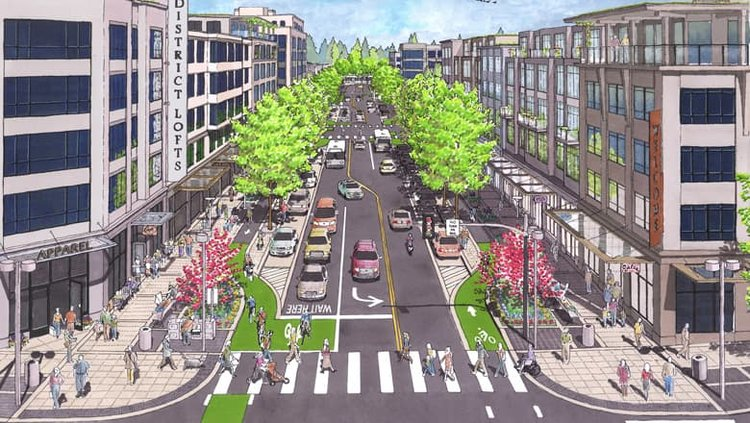
\includegraphics[width=0.65\linewidth]{images/complete_street_drawing.jpg}
	\end{figure}
	
\end{frame}



\begin{frame}
	
	\textbf{Complete Streets:} 
	
	\vspace{2mm}
	
	e.g. YongeTOmorrow 
	
	\vspace{2mm}
	
	\begin{figure}
		\centering
		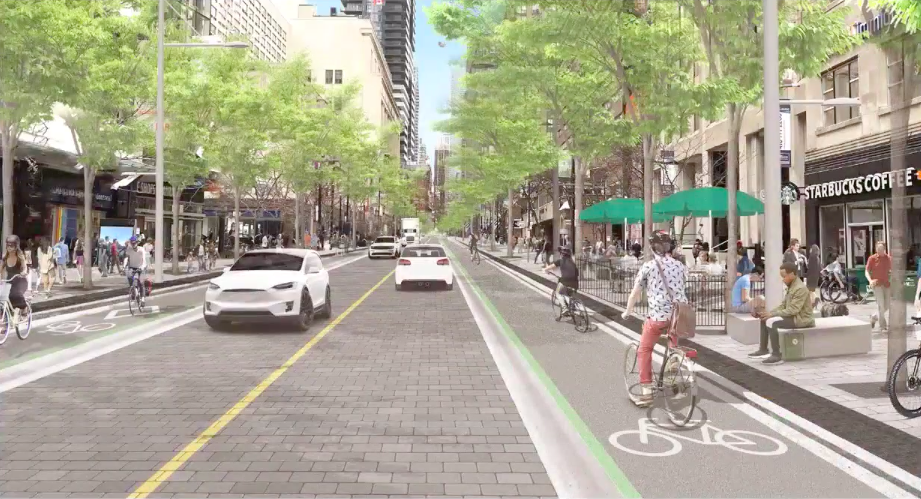
\includegraphics[width=0.85\linewidth]{images/yongetomorrow.png}
	\end{figure}
	
	\tiny\url{https://urbantoronto.ca/news/2021/01/downtown-yonge-makeover-finalized-heads-february-council-vote}
	
	
\end{frame}




\begin{frame}
	
	\textbf{Re-designing streets is difficult:} Can be differing public opinions
	
	\vspace{2mm}
	
	
	
		
	
	\begin{columns}
		\begin{column}{0.35\textwidth}
			
			e.g. this intersection was re-designed by local residents - then the city added temporary infrastructure - and then local residents voted to return to the original design
			
			\vspace{2mm}
			
			\tiny\url{https://www.cbc.ca/news/canada/toronto/dave-meslin-sidewalk-toronto-chalk-leaves-1.4427663}
			
			\vspace{2mm}
			
			\tiny\url{https://www.toronto.ca/wp-content/uploads/2019/07/8edc-Regal-Road-Consultation-Report-FINAL-AODA-July2019.pdf}
			
			
			
		\end{column}
		
		\begin{column}{0.65\textwidth}
			\begin{figure}
				\centering
				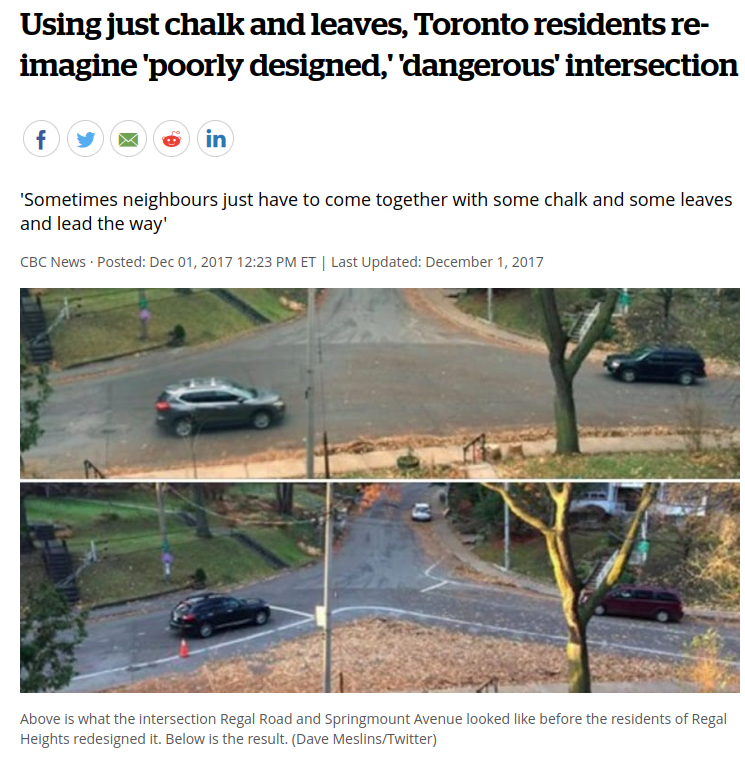
\includegraphics[width=0.9\linewidth]{images/leaves_road.png}
			\end{figure}
			
			
			
		\end{column}
		
		
		
	\end{columns}
	
	
\end{frame}




\begin{frame}
	
	\textbf{Re-designing streets is difficult:} Varying institutional interests
	
	

	\begin{figure}
		\centering
		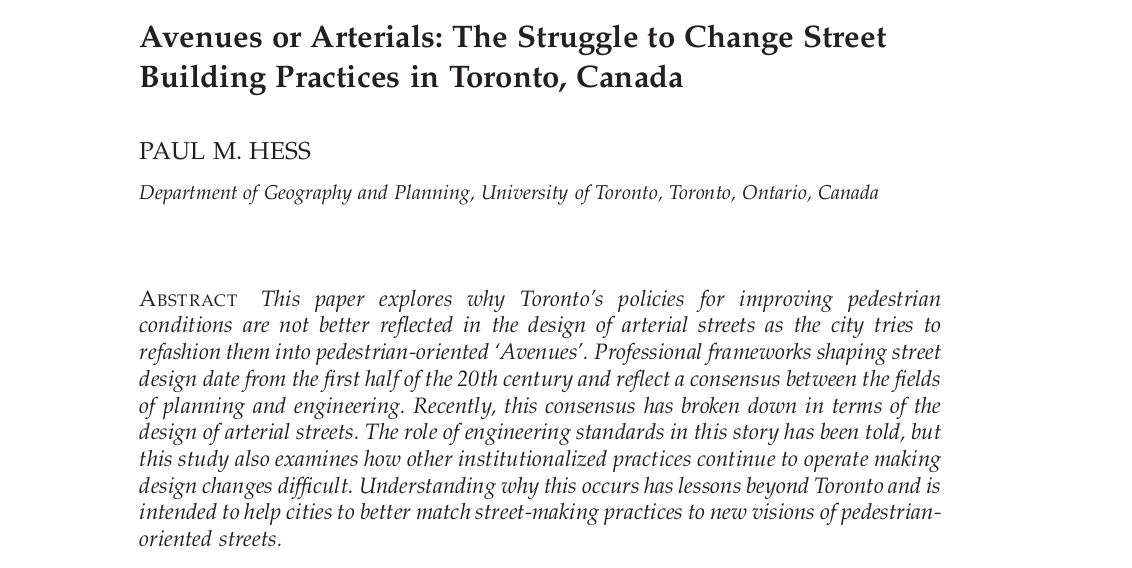
\includegraphics[width=0.9\linewidth]{images/avenues_or_arterials.png}
	\end{figure}
	
	\tiny{Hess, P. (2009) Avenues or Arterials: The struggle to change street building practices in Toronto, Canada. Journal of Urban Design, 14(1)}
	
\end{frame}




\begin{frame}
	
	\textbf{Re-designing streets is difficult:}
	
	\begin{itemize}
		\item Existing streets typically have a set ROW (Right of Way) width
		\item (re)design often involves trade-offs and competition for space
		\item e.g. competition between modes, as a place or for traffic flow, an avenue or an arterial, etc.
	\end{itemize}
	

	
	
	
%	\begin{itemize}
%		\item Streets as zero-sum game
%		
%		\item Place or Flow
%		
%		\item Avenues or Arterials:
%		
%		\item People or Cars:
%		
%	\end{itemize}
	
	
	\begin{figure}
		\centering
		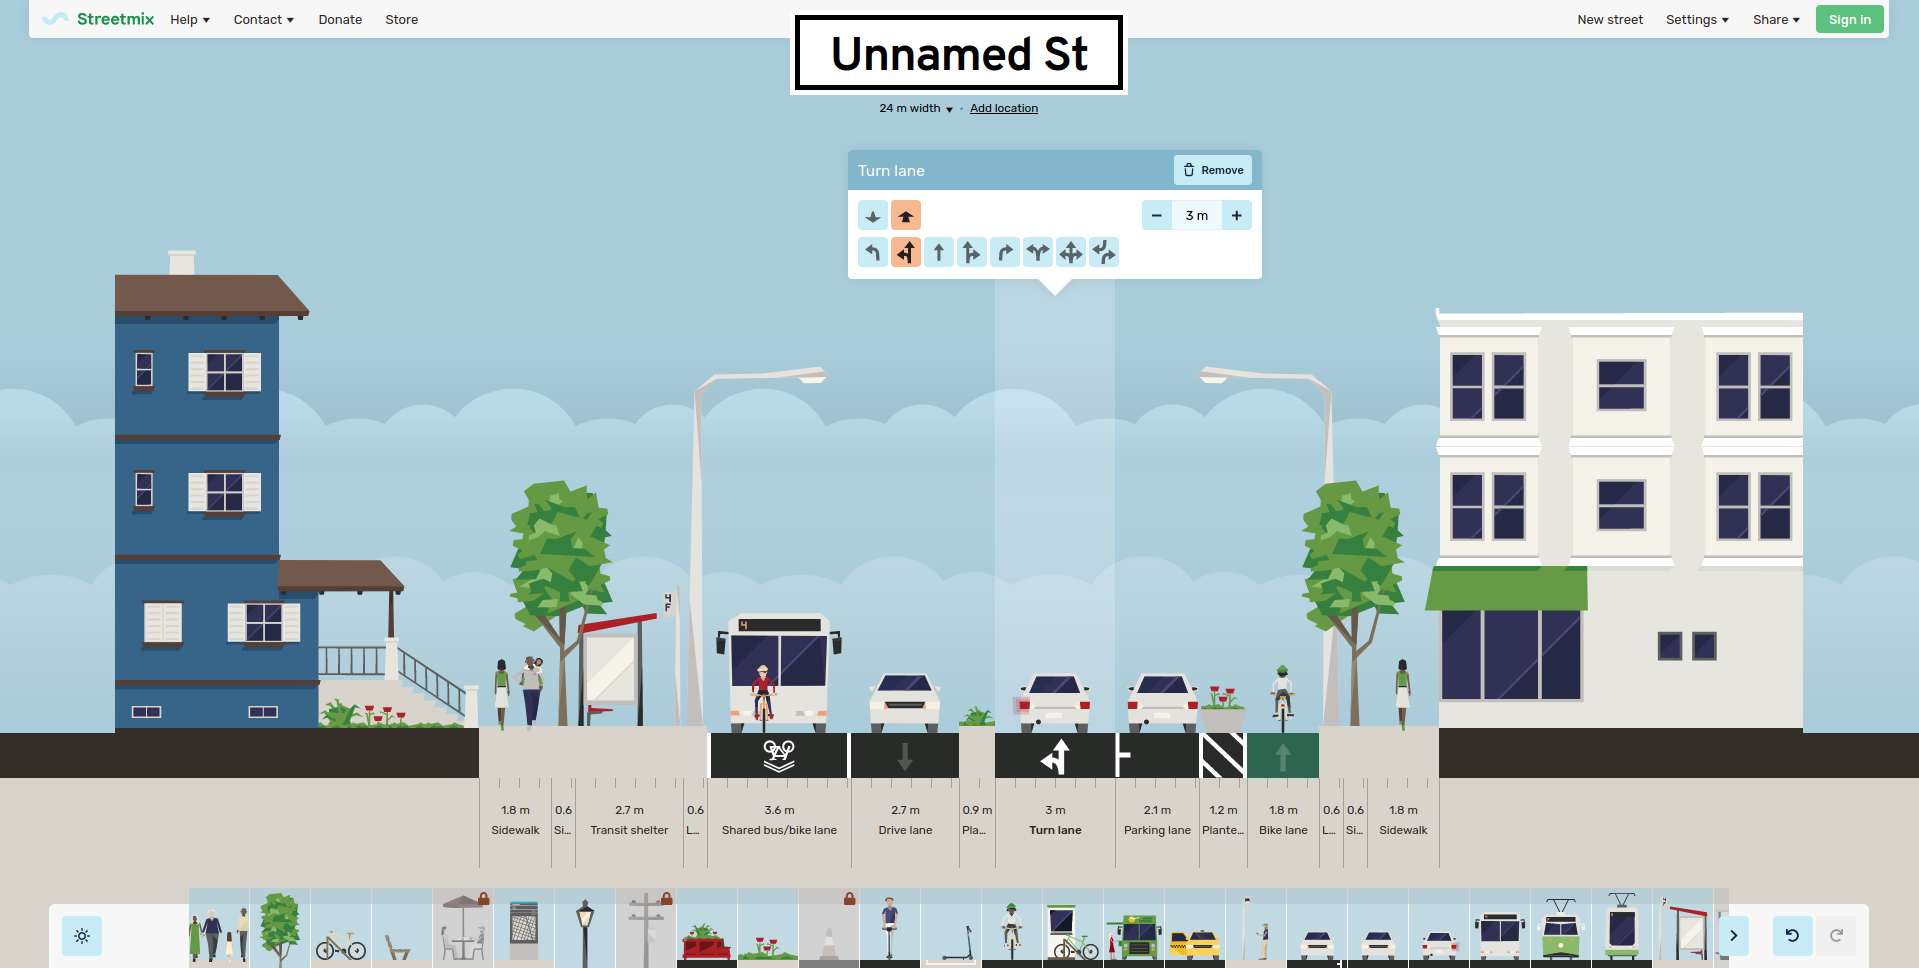
\includegraphics[width=0.85\linewidth]{images/streetmix.png}
	\end{figure}
	
	\tiny\url{https://streetmix.net}
	
\end{frame}






\begin{frame}
	
	\textbf{Street Re-Design Activity}


	\vspace{4mm}
	
	\begin{itemize}
		\item Queen Street West (Dufferin to Yonge) - 20m ROW
		\item University Ave (Queen to College) - 55m ROW
		\item Dufferin St South (Queen to Bloor) - 20m ROW
		\item Jane St North (Eglinton to Sheppard) - 27m ROW
		\item Lawrence East (Victoria Park to Kingston) - 36m ROW
	\end{itemize}

	
	\vspace{4mm}
	
	
	\begin{itemize}
		\item Use Google Streetview to briefly explore and describe current use (number of lanes, transit routes, bike lanes if they exist, etc.)
		\item Use Streetmix to re-design the street to make it more "complete"
	\end{itemize}
	
\end{frame}



\begin{frame}
	
	\textbf{Reducing barriers to active travel:} Improving Network Connectivity
	
	\begin{figure}
		\centering
		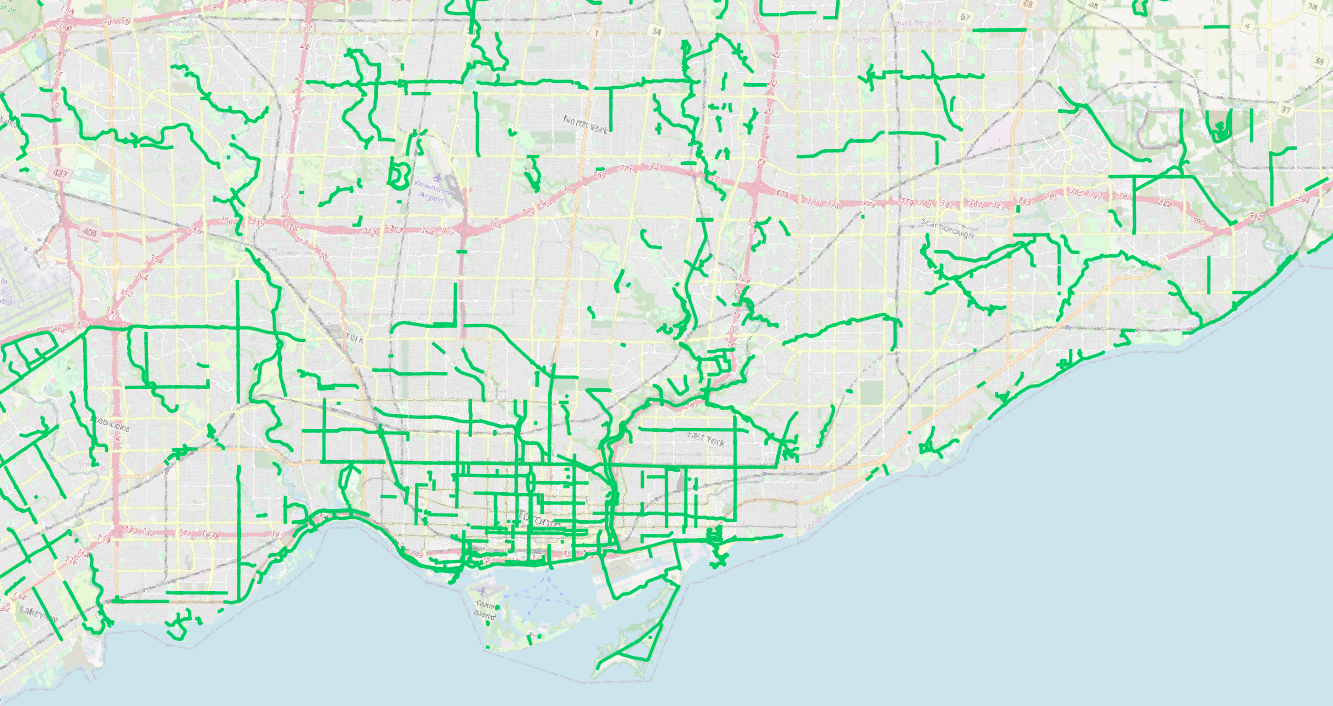
\includegraphics[width=1\linewidth]{images/bike_network_tor.png}
	\end{figure}
	
	\tiny From \url{https://www.openstreetmap.org}
	
\end{frame}


\begin{frame}
	
	\textbf{Reducing barriers to active travel:} Improving Network Connectivity
	
	\begin{figure}
		\centering
		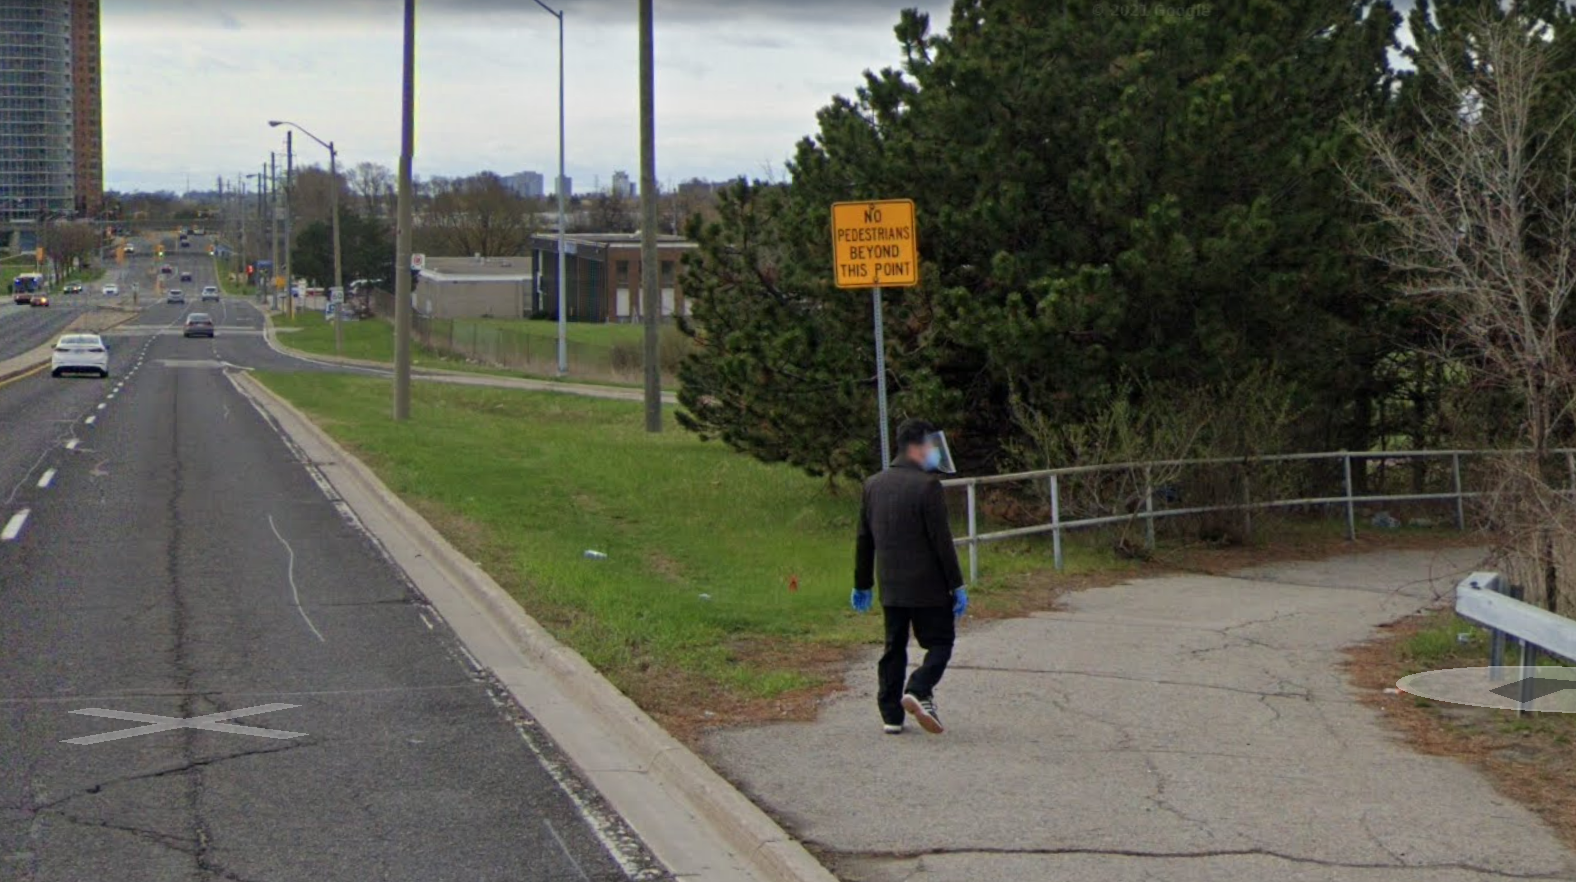
\includegraphics[width=1\linewidth]{images/brimley.png}
	\end{figure}
	
	\tiny Image from Google Streetview 
	\url{https://www.google.ca/maps/@43.7786041,-79.2645439,19z}
	
\end{frame}



\begin{frame}
	
	
	
	
	
	

	
	\begin{columns}
		\begin{column}{0.5\textwidth}
			
				\textbf{Reducing barriers to active travel:} 
			
				Blocking auto travel, but allowing bikes and pedestrians to travel through
			
			
				\begin{figure}
					\centering
					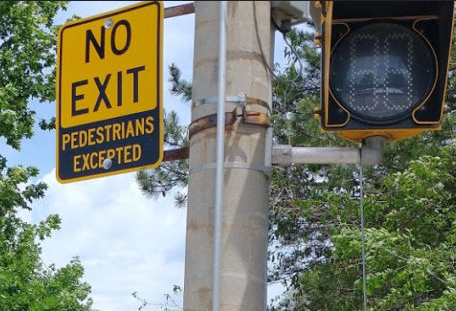
\includegraphics[width=1\linewidth]{images/no_exit.png}
				\end{figure}
		\end{column}
		
		\begin{column}{0.5\textwidth}
			\begin{figure}
				\centering
				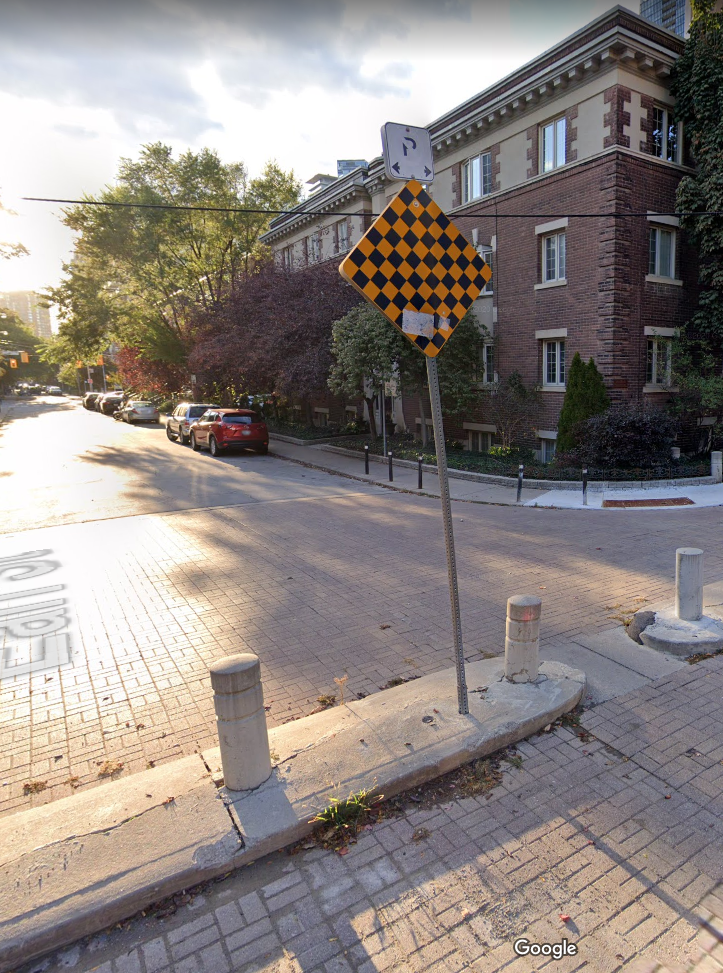
\includegraphics[width=0.9\linewidth]{images/earl_bike.png}
			\end{figure}
			
		\end{column}
		
		
		
	\end{columns}
	
	
\end{frame}



\begin{frame}
	
	\textbf{Reducing barriers to active travel:} Super Blocks
	
	\begin{figure}
		\centering
		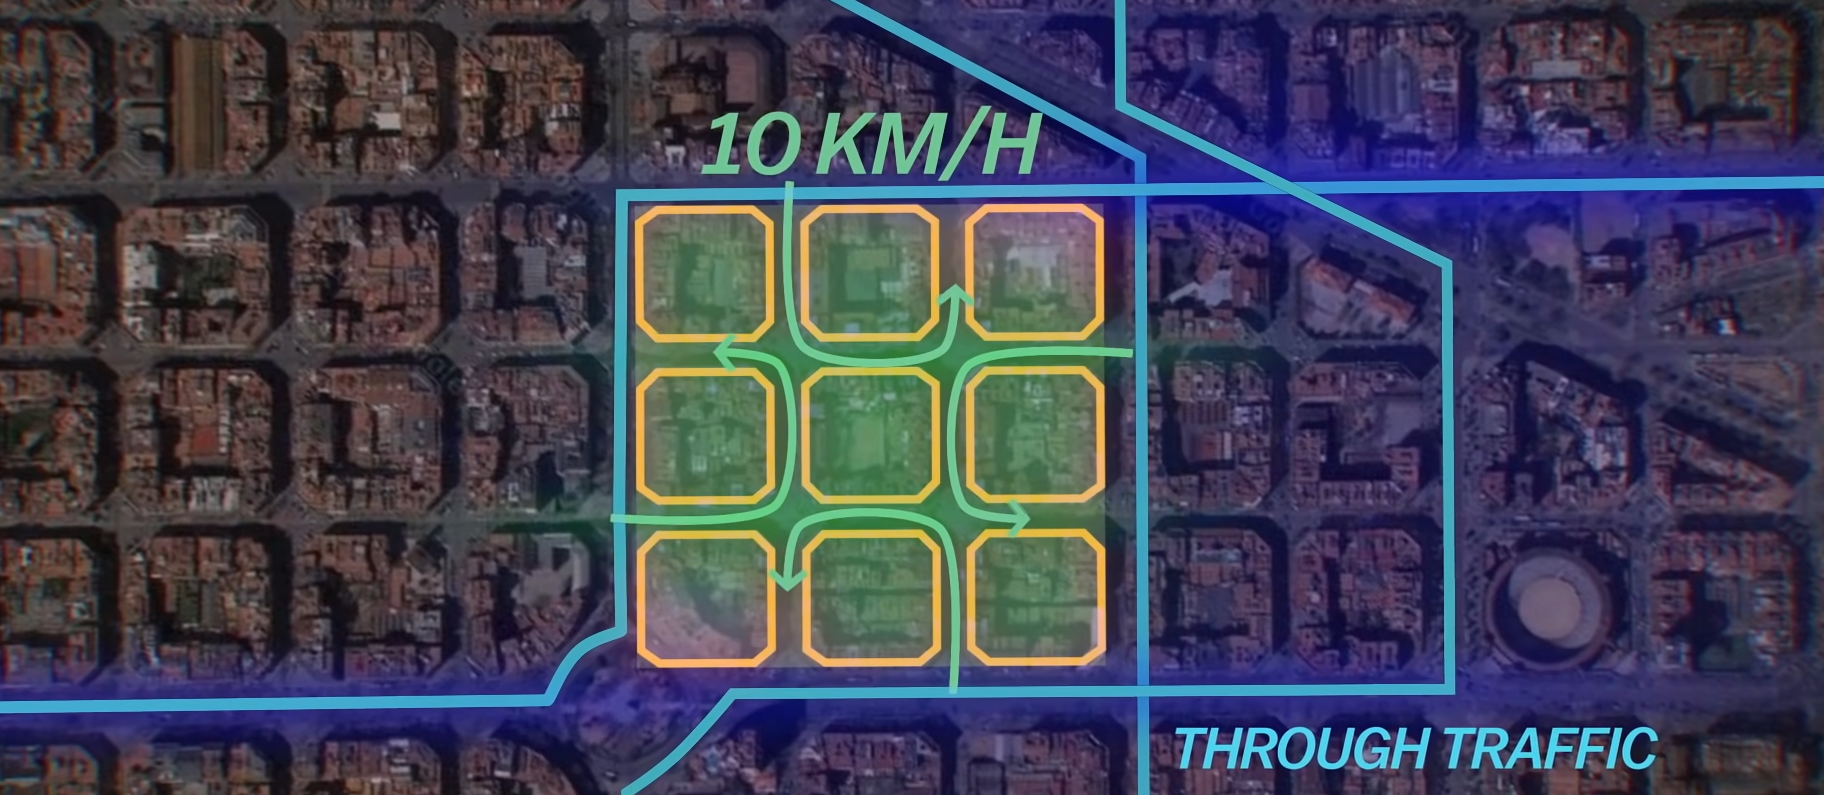
\includegraphics[width=0.8\linewidth]{images/super_blocks.png}
	\end{figure}
	
	\tiny 
	\url{https://www.archdaily.com/796252/how-barcelonas-superblocks-pedestrian-plan-hopes-to-return-the-streets-to-the-people}
	
	
	
\end{frame}



\begin{frame}
	
	\textbf{Reducing barriers to active travel:} Land-use and destination accessibility
	
	\vspace{2mm}
	
	e.g. there is a network of paths, but many destinations are really far away
	
	\begin{figure}
		\centering
		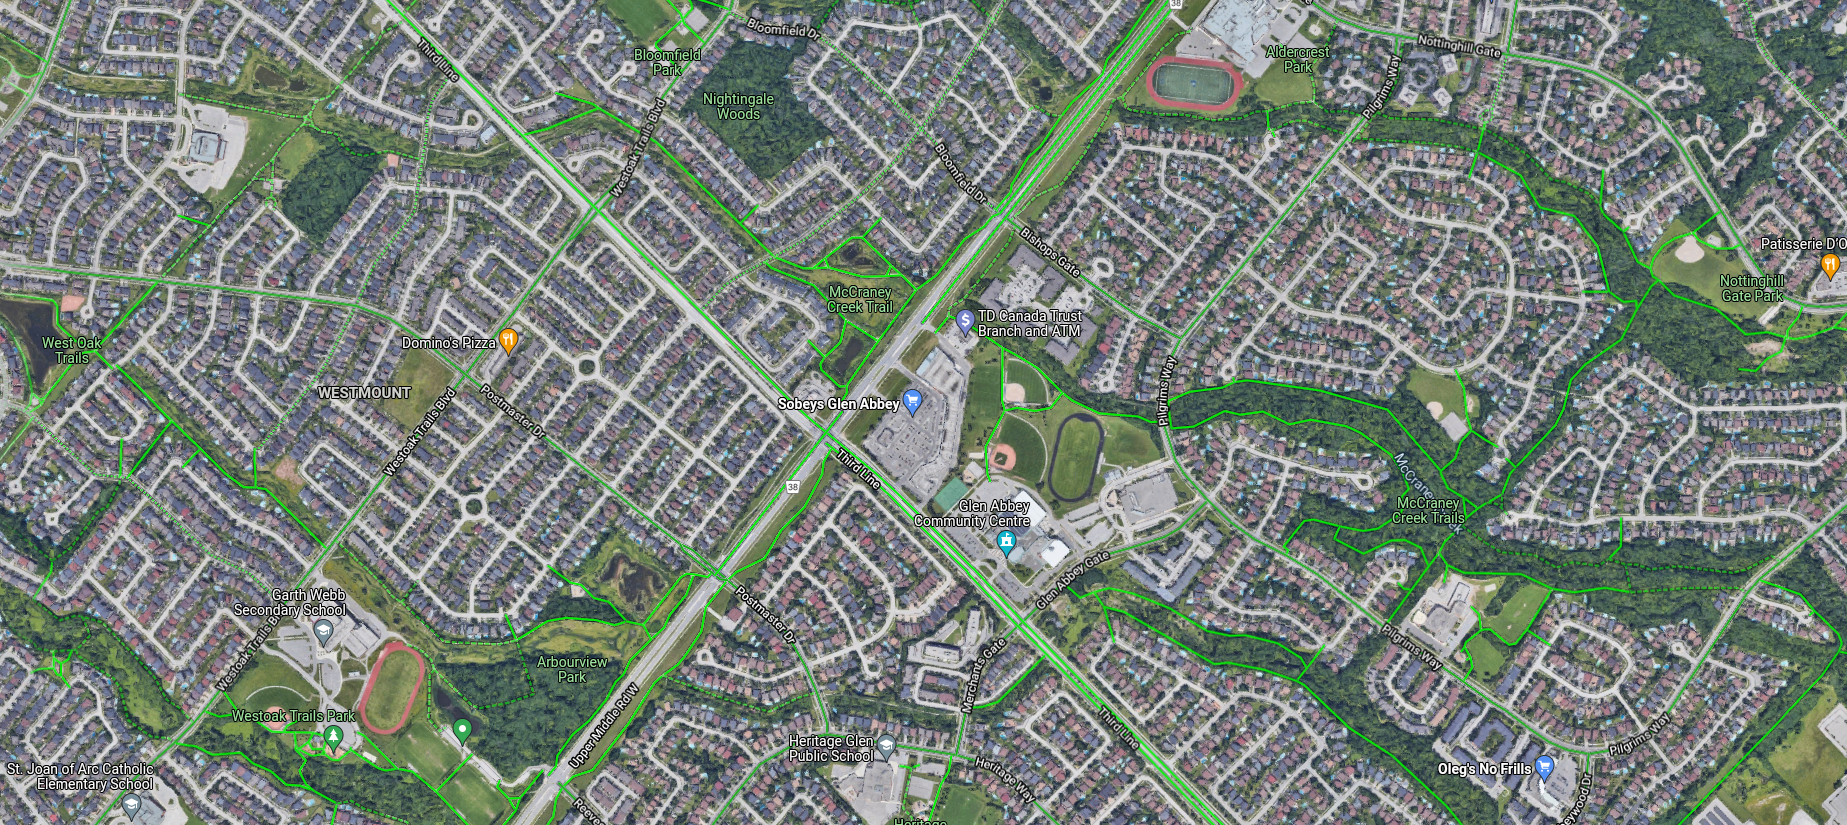
\includegraphics[width=1\linewidth]{images/suburb_bike_lanes.png}
	\end{figure}
	
%	\small 
%	
%	15-minute cities - most daily necessities can be reached by either walking or cycling (within 15 min)
%	
%	\vspace{2mm}
%	
%	We'll get into talking about measuring and evaluating accessibility in a couple weeks:
		
\end{frame}




\begin{frame}
	\textbf{Next Week} 
	
	\vspace{4mm}
	
	Public Transit
	
	\begin{itemize}
				
		
		\item Theory and practice of public transportation planning, design, and operations. 
		
		\item Overview of Transit Oriented Development (TOD)
		
	\end{itemize}
	
\end{frame}




\end{document}